%\setcounter{MaxMatrixCols}{30}

\documentclass{article}%
\usepackage{amsmath}
\usepackage{amsfonts}
\usepackage{amssymb}
\usepackage[margin=1in]{geometry}
\usepackage{graphicx}
\usepackage[numbers]{natbib}
\usepackage{cleveref}%
\setcounter{MaxMatrixCols}{30}

%\usepackage{algorithm2e}
\usepackage{algpseudocode}
\usepackage{algorithm}
\usepackage{xcolor}
\usepackage{url}
%TCIDATA{OutputFilter=latex2.dll}
%TCIDATA{Version=5.50.0.2960}
%TCIDATA{CSTFile=40 LaTeX article.cst}
%TCIDATA{Created=Thursday, January 09, 2025 15:40:48}
%TCIDATA{LastRevised=Friday, March 28, 2025 09:18:44}
%TCIDATA{<META NAME="GraphicsSave" CONTENT="32">}
%TCIDATA{<META NAME="SaveForMode" CONTENT="1">}
%TCIDATA{BibliographyScheme=Manual}
%TCIDATA{<META NAME="DocumentShell" CONTENT="Standard LaTeX\Blank - Standard LaTeX Article">}
%BeginMSIPreambleData
\providecommand{\U}[1]{\protect\rule{.1in}{.1in}}
%EndMSIPreambleData
\newtheorem{theorem}{Theorem}[section]
\newtheorem{acknowledgement}[theorem]{Acknowledgement}
%\newtheorem{algorithm}[theorem]{Algorithm}
\newtheorem{assumption}[theorem]{Assumption}
\newtheorem{axiom}[theorem]{Axiom}
\newtheorem{case}[theorem]{Case}
\newtheorem{claim}[theorem]{Claim}
\newtheorem{conclusion}[theorem]{Conclusion}
\newtheorem{condition}[theorem]{Condition}
\newtheorem{conjecture}[theorem]{Conjecture}
\newtheorem{corollary}[theorem]{Corollary}
\newtheorem{criterion}[theorem]{Criterion}
\newtheorem{definition}[theorem]{Definition}
\newtheorem{example}[theorem]{Example}
\newtheorem{exercise}[theorem]{Exercise}
\newtheorem{lemma}[theorem]{Lemma}
\newtheorem{notation}[theorem]{Notation}
\newtheorem{problem}[theorem]{Problem}
\newtheorem{proposition}[theorem]{Proposition}
\newtheorem{remark}[theorem]{Remark}
\newtheorem{solution}[theorem]{Solution}
\newtheorem{summary}[theorem]{Summary}
\newenvironment{proof}[1][Proof]{\noindent\textbf{#1.} }{\ \rule{0.5em}{0.5em}}



\DeclareMathOperator{\supp}{supp}
\newcommand{\R}{\mathbb{R}}
\newcommand{\E}{\mathbb{E}}
\newcommand{\Prob}{\mathbb{P}}
\newcommand{\dd}{\,\mathrm{d}}
\newcommand{\thetahat}{\hat{\theta}_n}
\newcommand{\thetastar}{\theta^*}
\newcommand{\one}{\boldsymbol{1}}
\newcommand{\Leb}{\mathrm{Leb}}
\newcommand{\Lap}{\mathrm{Lap}}
\newcommand{\diff}{\mathrm{d}}
\newcommand{\1}{\mathbf{1}}

\begin{document}

\title{Bayes-assisted anytime-valid t-tests and confidence sequences for Gaussian means with unknown variance}
\author{Debolina Paul, Patrick Rebeschini, Fran\c{c}ois Caron}
\maketitle

\begin{abstract}

We propose an anytime-valid test of $H_0:\mu=0$ versus $H_1:\mu\neq 0$ for i.i.d.\ normal data with unknown variance, using prior information on the standardized effect size $\delta=\mu/\sigma$. The test mixes a scale-invariant likelihood ratio over a prior on $\delta$ and applies the extended Ville inequality to obtain a valid p-process under arbitrary stopping. When the prior is well specified, the method improves power for alternatives favoured by the prior. For every fixed $n$ and dataset, if the prior has polynomial tails and is centered at $m$, then we show that the time-$n$ p-value converges to the anytime-valid $t$-test p-value as $m\to\infty$. Thus the procedure gains power when the prior is accurate and reverts to the non-informative benchmark under extreme prior-data conflict.

\end{abstract}

keywords: p process; extended Ville inequality; power-law tails; method of mixtures 

\section{Introduction}
\label{sec:intro}
Classical statistical inference assumes that the sample size \(n\) is
fixed before the data are seen. The familiar guarantees of fixed-sample
\(p\)-values and confidence intervals, \(\mathbb{P}_{H_0}(p_n \leq \alpha) \leq \alpha\), \(\mathbb{P}_\theta(\theta \in C_n) \geq 1-\alpha\) hold for each \(n\) separately, but degrade arbitrarily when the sample size is itself a function of the data. 
\cite{wagenmakers2007practical} and \cite{simmons2011false} document how
data-dependent stopping i.e. checking the \(p\)-value after each new
observation and continuing if it is above \(\alpha\) inflates Type I
error far beyond the nominal level, and is a quantitatively important
contributor to the reproducibility crisis in the experimental sciences.
The methodological response, developed over the last decade, has been the framework of anytime-valid inference testing procedures whose error
guarantees hold uniformly over all stopping rules, including the
adversarial rule to stop as soon as the result looks significant
\citep{Howard2021, grunwald2020safe, RamdasGrunwald2023}. The technical core of this framework is the construction of a non-negative martingale, supermartingale, or \(e\)-process \((M_n)_{n\geq 1}\) adapted to the data with \(M_0=1\) and \(\E_{H_0}[M_n]\leq 1\) for all \(n\). Ville's inequality \citep{ville1939etude} then gives \(\mathbb{P}_{H_0}(\exists n: M_n \geq 1/\alpha) \leq \alpha\), and rejecting \(H_0\) when \(M_n\) first crosses \(1/\alpha\) yields a test that is valid at every stopping time simultaneously. Inverting the test produces a confidence
sequence \(C_{\alpha,n}\) covering the true parameter with probability
at least \(1-\alpha\) uniformly in \(n\) \citep{Darling1967, Robbins1970, Lai1976}.

A parallel literature, motivated by the Bayesian reanalysis of
psychological experiments, has developed informative analogues of the
\(t\)-test based on prior distributions on the standardised effect size
\(\delta=\mu/\sigma\). The Jeffreys-Zellner-Siow (JZS) Bayes factor of
\cite{Rouder2009}, building on \cite{jeffreys1998theory} and
\cite{zellner1980posterior}, places a Cauchy prior on \(\delta\) and
integrates the right-Haar prior \(\sigma^{-1}\dd\sigma\) over \(\sigma\),
yielding a closed-form Bayes factor in terms of the parabolic cylinder
function. The Cauchy choice is motivated by Jeffreys's robustness
argument: among location-scale families, only priors with polynomial
tails ensure that the Bayes factor does not collapse to extreme values
when the observed effect is much larger than the prior anticipated.
This robustness motivation has spawned a wide literature on
heavy-tailed priors for the \(t\)-test, the horseshoe family
\cite{Carvalho2010}, generalised Student-\(t\) priors \cite{gronau2020informed}, mixtures of \(g\)-priors, all of which are recognised, from the anytime-valid perspective, as different choices of mixing distribution in the same fundamental construction. What distinguishes the anytime-valid reading of these Bayes factors is the observation, due to \cite{PerezOrtiz2024} and \cite{Wang2025}, that the JZS Bayes factor is itself a non-negative martingale on the scale-invariant filtration: the Bayes factor of \cite{Rouder2009} is, after appropriate calibration, an anytime-valid \(p\)-process.

The use of informative priors raises an obvious robustness question, but
what happens when the prior is wrong? In the known-variance setting,
\cite{Cortinovis2025} showed that the natural answer is delicate. Mixing
against an informative prior tightens the confidence sequence under
prior-data agreement, but the volume of the classical Ville confidence
sequence diverges as the conflict between the prior and the data
grows, rendering the procedure vacuous. Their remedy combines the
extended Ville inequality of \cite{wang2025extended} with priors having
polynomial or exponential tails. The result is a procedure that is
sharper than the non-informative benchmark when the prior is correct,
yet crucially reverts smoothly to the non-informative procedure
under arbitrary prior-data conflict. This bounded-influence property is structurally tied to the tail behaviour of the prior: heavy-tailed priors absorb conflict, light-tailed priors do not. The
framework of \cite{Cortinovis2025} thereby provides a principled way to
incorporate prior information without paying a robustness price in the
worst case, and tries to connect the anytime-valid \(t\)-test literature to
the classical Bayesian-robustness tradition of \cite{Dawid1973, PericchiSmith1992, PericchiSanso1995, Berger1980}.

\cite{Cortinovis2025} however treats the case where the variance \(\sigma^2\) is
known. The unknown-variance case is the practically important one, this is where the \(t\)-test framework is needed in the first place and is the main contribution of this report. We present a unified development of the anytime-valid \(t\)-test with informative priors, combining the mixture-martingale constructions of \cite{Lai1976} and \cite{Wang2025} with the bounded-influence framework of \cite{Cortinovis2025}. We obtain closed-form expressions for the mixture statistic under the Lebesgue prior, recovering the scale-invariant \(t\)-statistic of \cite{Lai1976}, and under one-sided exponential tilts in terms of the parabolic cylinder function, characterise the directional limits of the symmetric Laplace mixture, prove that the classical Ville confidence sequence is fragile under prior-data conflict for every proper prior, and establish a Lebesgue-recovery theorem for polynomial-tail priors. We would like to complement these results by theoretically exhibiting a third regime, sub-Gaussian priors in which the procedure fails to reject regardless of the data, as observed in the simulations. We have also proved an obstruction to a Hausdorff-type data-conflict theorem that exists in the known-variance setting but not in the
unknown-variance setting. Together, the results trace out a trichotomy of tail behaviours for the prior: heavy-tailed (polynomial) priors recover the non-informative benchmark, intermediate (exponential) priors land at a directionally informative limit, and light-tailed (sub-Gaussian) priors break the procedure entirely.


\subsection{Notation}

For \(a,b\in\mathbb{R}\), \(a\wedge b=\min(a,b)\). For a probability measure
\(\Pi\) on \(\mathbb{R}\) and \(m\in\mathbb{R}\), let \(\Pi_m\) denote the
location-shifted measure with density \(\pi_m(\theta)=\pi(\theta-m)\),
when a density \(\pi\) exists. We write \(f(x)\sim g(x)\) as
\(x\to a\) for \(\lim_{x\to a} f(x)/g(x)=1\). %The Hausdorff distance
%between two closed subsets \(C_1,C_2\subset\R\) is denoted \(d_H\).
\(\chi_n\) denotes the chi distribution with \(n\) degrees of freedom
and \(\chi_n^2\) its square. \(D_{-n}\) is the parabolic cylinder
function\footnote{\url{https://en.wikipedia.org/wiki/Parabolic_cylinder_function}}.

\section{Setup and background}\label{sec:setup}
\subsection{Anytime-valid testing}

Let \(Y_1,Y_2,\ldots\) be i.i.d.\ \(\mathcal N(\mu,\sigma^2)\) with
\(\mu\in\mathbb{R}\) and \(\sigma>0\) both unknown, and write
\(\theta^\star=\mu/\sigma\). For \(\theta_0\in\mathbb{R}\) we consider the
composite testing problem
\begin{equation}\label{eq:tests}
   H_0\!:\theta^\star=\theta_0 \qquad\text{vs}\qquad
   H_1\!:\theta^\star\neq\theta_0.
\end{equation}
This relies on the construction of a sequence of anytime-valid p-values, or p-process, $(P_{n,\theta_0})_{n\geq 1}$, where $P_{n,\theta_0}:=P_{n,\theta_0}(Y_{1:n})$, that satisfies, for any $\alpha\in (0,1)$
\begin{equation}\label{eq:pprocess}
   \Prob_{H_0}\!\bigl(\exists n\geq 2:\, P_{n,\theta_0}\leq \alpha\bigr)
   \leq \alpha.
\end{equation}
The test then rejects $H_0$ if $P_{k,\theta_0}\leq \alpha$ for some $k\leq n$. 

Inverting a family \((P_{n,\theta_0})_{n\geq 2,\theta_0\in\mathbb{R}}\) yields
a \emph{confidence sequence}
\begin{equation}\label{eq:CS-from-pproc}
   C_{\alpha,n}(y_{1:n})
   \;=\;\bigl\{\theta_0\in\mathbb{R}\,:\,P_{n,\theta_0}(y_{1:n})>\alpha\bigr\},
\end{equation}
which satisfies
\(\Prob(\theta^\star\in C_{\alpha,n}(Y_{1:n})\text{ for all
}n\geq 2)\geq 1-\alpha\).

\subsection{Confidence sequence}

Using now a family of p-processes $((P_{n,\theta_0})_{n\geq 1})_{\theta_0\in\mathbb R}$, one can obtain a confidence sequence for the parameter $\theta^*$ by inversion of the family of tests \eqref{eq:tests}:
$$
C_{\alpha,n}(Y_{1:n})=\left\{ \theta_0 \mid P_{n,\theta_0}> \alpha\right \}.
$$
By the above properties of the p-process (Equation \eqref{eq:pprocess}), the sequence $(C_{\alpha,n}(Y_{1:n}))_{n \geq 1}$ is a confidence sequence, satisfying
$$
\mathbb P(\theta^*  \in C_{\alpha,n}(Y_{1:n}) \text{ for all }n\geq 2)\geq 1-\alpha.
$$

The unifying object behind all anytime-valid procedures considered in
this report is a non-negative process \((M_n)_{n\geq 1}\) that is a
martingale of mean one under \(H_0\): \(\E_0[M_{n+1}\mid\mathcal{F}_n]
=M_n\) with \(\E_0[M_1]=1\). Such a process has the interpretation of a
gambler's wealth in a fair game against \(H_0\): starting with one
unit, the gambler bets on each new observation, and the martingale
property says the game is fair under the null. The intuition behind
anytime validity is then transparent, if \(H_0\) is true the gambler
cannot get rich, so the event ``wealth ever exceeds \(1/\alpha\)" must
have probability at most \(\alpha\). This is precisely Ville's
inequality, and rejecting \(H_0\) when the wealth crosses \(1/\alpha\)
gives a test that is valid at every stopping time simultaneously.

\subsection{(Extended) Ville's inequality and the method of mixtures}

The starting point is \cite{ville1939etude}'s inequality, together with its recent extension to nonintegrable nonnegative supermartingales
\citep{wang2025extended}.

\begin{proposition}[Ville's inequality]\label{prop:ville}
Let \((X_n)_{n\geq 1}\) be a nonnegative martingale with
\(\E[X_1]=1\). Then for any \(\alpha\in(0,1]\),
\(\Prob\bigl(\sup_{n\geq 1} X_n\geq 1/\alpha\bigr)\leq\alpha\).
\end{proposition}

\begin{proposition}[Extended Ville's inequality;
{\cite[Thm.~4.1]{wang2025extended}}]
\label{prop:eville}
Let \((X_n)_{n\geq 1}\) be an extended nonnegative supermartingale.
For any \(c>0\),
\[
   \Prob\left(\sup_{n\geq 1} X_n\geq c\right)\;\leq\;
   \E\!\bigl[\min(X_1/c,\,1)\bigr].
\]
\end{proposition}

If \((M_n(Y_{1:n};\theta_0))_{n\geq 2}\) is an (extended) nonnegative
martingale under \(H_0:\theta^\star=\theta_0\) with respect to a
suitable filtration, then
\(P_{n,\theta_0}=g_{\theta_0}\bigl(M_n(Y_{1:n};\theta_0)\bigr)\)
defines a valid p-process, where
\begin{equation}\label{eq:gtheta0}
  g_{\theta_0}(c)\;=\;
   \begin{cases}
     1/c, & \text{(Ville)},\\[2pt]
     \E_{\theta_0}\!\bigl[\min(M_2(Y_{1:2};\theta_0)/c,\,1)\bigr],
       & \text{(extended Ville)}.
   \end{cases}
\end{equation}

The classical Ville inequality requires the process
\((X_n)\) to be integrable with \(\E_0[X_1]\leq 1\), which corresponds
in the mixture construction~\eqref{eq:Mn-def} to a proper prior \(\Pi_0\). Many priors of practical interest are not proper, such as the Lebesgue prior \(\Pi_{\mathrm{Leb}}\), the one-sided
exponential tilt etc. The location-shifted polynomial-tail priors are
proper but lead to mixture statistics whose unconditional expectation
under \(\mathbb{P}_0\) diverges as the prior is shifted far from the origin. In all these cases, the mixture process is still a non-negative
martingale of mean one if interpreted on the right filtration, but its
unconditional initial value \(\E_0[M_2]\) is infinite, and the
classical Ville inequality is vacuous.

The extended Ville inequality \citep{wang2025extended} resolves this by replacing the classical bound \(1/c\) with \(\E_0[\min(M_2/c,1)]\),
which is always at most one regardless of integrability. The trade-off
is that the calibration function \(g(c)=\E_0[\min(M_2/c,1)]\) must be
evaluated under \(\mathbb{P}_0\), typically by Monte Carlo if no closed form is available. The price of improperness is therefore not a loss of
validity, but a computational overhead in calibration.

\subsection{Scale invariance and the maximal-invariant statistic}
The model \(Y_1,\ldots,Y_n\stackrel{\mathrm{iid}}{\sim}\mathcal{N}(\mu,\sigma^2)\)
has an obvious symmetry: rescaling \(Y_i\mapsto cY_i\) for \(c>0\)
sends \((\mu,\sigma)\mapsto(c\mu,c\sigma)\) but leaves the ratio
\(\theta^\star=\mu/\sigma\) unchanged. An inferential procedure that
respects the units of measurement of \(Y\) must therefore depend on
the data only through scale-invariant functions, and on the parameter
only through \(\theta^\star\). The two are linked: \((\mu,\sigma)\) is
identifiable only up to this symmetry, and \(\theta^\star\) is the
unique identifiable quantity.

This identifiability constraint determines almost the entire
construction that follows. First, the right object to test is
\(H_0:\theta^\star=\theta_0\), not \(H_0:\mu=\mu_0\), since the latter
is not scale-equivariant. Second, the right filtration to work with is
not \((\sigma(Y_1,\ldots,Y_n))_n\) but the smaller scale-invariant
filtration \(\mathcal{F}_n=\sigma(Z_1,\ldots,Z_n)\), \(Z_i=Y_i/|Y_1|\),
which strips out \(\sigma\) while retaining every scale-invariant
function of the data. The statistics \(Z_{1:n}\) are a maximal-invariant statistic for the action of the scale group, meaning that two data vectors give the same \(Z_{1:n}\) iff they are scale-related, and any scale-invariant function of the data factorises through \(Z_{1:n}\).

The likelihood ratio on \(\mathcal{F}_n\) admits two equivalent
representations: as a likelihood ratio on the maximal invariant
itself, and as the integrated likelihood under the right-Haar measure
\(\sigma^{-1}\dd\sigma\) on the scale parameter. Equation~(5) shows this as the LHS is the maximal-invariant LR while the RHS is the
right-Haar-marginalised LR. Their equality is a classical identity in
group-invariant inference~\citep{eaton1989group, lehmann2005testing}. The right-Haar measure
plays this role because it is invariant under the group action, so
integrating it out produces a function of the maximal invariant. This
identity is the reason the scale-invariant likelihood ratio \(L_n\) of
equation~\eqref{eq:scale-inv-LR} is computable in closed form even though \(\sigma\) is unknown.


\subsection{Scale-invariant likelihood ratios}\label{ssec:scale-inv}

In our model the parameter \(\sigma\) is a nuisance scale parameter.
We therefore consider the scale-invariant filtration generated by the
ratios \(Z_i=Y_i/|Y_1|\), \(i\geq 1\), and the corresponding
maximal-invariant statistic. Let
\(\eta_{n,\theta}(z_{1:n})\) denote the joint density of
\((Z_1,\ldots,Z_n)\) under \(\Prob_\theta\) (which is independent of
\(\sigma\)). For any \(\theta,\theta_0\in\mathbb{R}\) and \(n\geq 1\), define
\begin{equation}\label{eq:scale-inv-LR}
  L_n(y_{1:n};\theta_0,\theta)
  \;=\;\frac{\eta_{n,\theta}(y_1/|y_1|,\ldots,y_n/|y_1|)}
            {\eta_{n,\theta_0}(y_1/|y_1|,\ldots,y_n/|y_1|)}
  \;=\;\frac{\int_0^\infty f_{n,\theta,\sigma}(y_{1:n})\sigma^{-1}\dd\sigma}
            {\int_0^\infty f_{n,\theta_0,\sigma}(y_{1:n})\sigma^{-1}\dd\sigma},
\end{equation}
where \(f_{n,\theta,\sigma}\) is the joint density of \(Y_{1:n}\)
under \(\mathcal N(\theta\sigma,\sigma^2)\). The right-hand side of
\eqref{eq:scale-inv-LR} expresses \(L_n\) as a likelihood ratio under
the right-Haar prior \(\sigma^{-1}\dd\sigma\), making \(L_n\) a
function of the maximal-invariant alone.

\cite{Wang2025} and also
\cite{PerezOrtiz2024} show that
\((L_n(Y_{1:n};\theta_0,\theta))_{n\geq 1}\) is a nonnegative
\((\mathcal F_n)\)-martingale of mean one under
\(\Prob_{\theta_0}\), where \(\mathcal F_n=\sigma(Z_1,\ldots,Z_n)\). A
direct computation \cite[Sec.~4.4]{Wang2025} yields
\begin{equation}\label{eq:hthetadef}
  L_n(y_{1:n};\theta_0,\theta)
  \;=\;\frac{h_{\theta,n}(y_{1:n})}{h_{\theta_0,n}(y_{1:n})},
  \qquad
  h_{\theta,n}(y_{1:n}) \;=\; e^{-n\theta^2/2}\,A_n\bigl(\theta\,u_n(y_{1:n})\bigr),
\end{equation}
where
\begin{align}
  A_n(z) &\;=\;\frac{1}{\Gamma(n/2)}\int_0^\infty y^{n/2-1}
                \exp\!\bigl(-y+z\sqrt{2y}\bigr)\dd y
              \;=\; \E\bigl[e^{z R_n}\bigr],\quad R_n\sim\chi_n,
              \label{eq:Andef}\\[2pt]
  u_n(y_{1:n})
       &\;=\;\frac{\sum_{i=1}^n y_i}{\sqrt{\sum_{i=1}^n y_i^2}}
       \;=\;\frac{n\widehat\theta_n}{\sqrt{(n-1)+n\widehat\theta_n^2}}
       \;\in\;[-\sqrt n,\sqrt n],
       \label{eq:undef}
\end{align}
and \(\widehat\theta_n=\bar Y_n/S_n\) is the sample Sharpe ratio
(with \(\bar Y_n=n^{-1}\sum Y_i\) and
\(S_n^2=(n-1)^{-1}\sum(Y_i-\bar Y_n)^2\)).
The statistic \(u_n\) is scale-invariant and equivalent to the
classical \(t\)-statistic. A detailed calculation is given in the Appendix \ref{app:a}.

\paragraph{Justification for convergence of $A_n$.} The integrand of $A_n(z)$ is locally integrable at $0$ because $y^{n/2-1}$ is integrable there for every $n\geq 1$ (as $n/2-1>-1$). At
infinity, the elementary bound $z\sqrt{2y}\leq y/2 + z^{2}$ (Young's inequality applied to $z\sqrt{2y}=\sqrt{2}z\cdot\sqrt{y}$) gives
\[
-y + z\sqrt{2y} \;\leq\; -y/2 + z^{2},
\]
so $A_n(z)\leq e^{z^{2}}\int_{0}^{\infty}y^{n/2-1}e^{-y/2}\diff y
= 2^{n/2}\Gamma(n/2)e^{z^{2}}<\infty$. The integral defining
$A_n(z)$ is therefore absolutely convergent for every $z\in\mathbb{R}$, and the order-of-integration manipulations used here are justified.


\subsection{Mixture construction}\label{ssec:mixture}

Let \(\Pi_0\) be a \(\sigma\)-finite measure on \(\mathbb{R}\). Define the
mixture martingale process
\begin{equation}\label{eq:Mn-def}
  M_n^{\Pi}(y_{1:n};\theta_0)
  \;=\;\int_\mathbb{R} L_n(y_{1:n};\theta_0,\theta)\,\Pi(\dd\theta)
  \;=\;\frac{\int_\mathbb{R} h_{\theta,n}(y_{1:n})\,\Pi(\dd\theta)}
            {h_{\theta_0,n}(y_{1:n})},
\end{equation}
provided the integral is finite. When \(\Pi\) is proper,
\((M_n^{\Pi}(Y_{1:n};\theta_0))_{n\geq 1}\) is a non-negative
martingale of mean one under \(\Prob_{\theta_0}\); and hence
\[
P_n^{V,\Pi}(y_{1:n})=\frac{1}{M_n^\Pi(y_{1:n})}
\]
is a valid Ville p-process.

For a general $\sigma$-finite $\Pi$ (in particular for an improper prior), the appropriate anytime-valid p-variable is the extended one as $(M_n^\Pi)_{n\geq 1}$ is an extended non-negative martingale \citep{wang2025extended},
\[
P_n^{E,\Pi}(y_{1:n})=g_\Pi(M_n^\Pi(y_{1:n})),
\qquad
g_\Pi(c)=\E_{0}\!\left[\min\!\left(\frac{M_2^\Pi(Y_{1:2})}{c},1\right)\right]
\]
where $\E_0$ denotes expectation under $H_0:\theta^*=0$.

In both
cases, the construction
\begin{equation}\label{eq:p-from-M}
  P_{n,\theta_0}(y_{1:n})
  \;=\;
  g_{\theta_0}\!\bigl(M_n^{\Pi_0}(y_{1:n};\theta_0)\bigr),
  \qquad n\geq 2,
\end{equation}
with \(g_{\theta_0}\) as in \eqref{eq:gtheta0}, defines an anytime-valid
p-process. The corresponding confidence sequences via
\eqref{eq:CS-from-pproc} are denoted by \(C^V_{\alpha,n}\) (Ville) and
\(C^{eV}_{\alpha,n}\) (extended Ville).

From the Bayesian perspective, \(M_n^{\Pi}\) is
the Bayes factor for \(H_0\) against the composite alternative
\(H_1:\theta^\star\sim\Pi_0\), evaluated under the right-Haar prior on
\(\sigma\). From the betting perspective, the prior \(\Pi\) is a strategy: it specifies how the gambler allocates wealth across the alternative directions \(\{\theta:\theta\neq\theta_0\}\), and the
process \(M_n^{\Pi_0}\) is the gambler's accumulated wealth from this
strategy. A prior concentrated on the true value of \(\theta^\star\)
makes the gambler rich quickly, yielding a powerful test; a misplaced
prior corresponds to a bad betting strategy, with consequences we
quantify in Section~\ref{sec:bdd-influence}.

\begin{remark}\label{rem:start-n2}
Under the Lebesgue prior, \(M_1^{\Pi_{\Leb}}=+\infty\) since
\(|u_1|=1=\sqrt 1\); hence the natural starting index for the
extended-Ville procedure is \(n=2\). Throughout the paper we adopt
the convention \(n\geq 2\).
\end{remark}

\section{Closed-form mixtures for $H_0:\theta^\star=0$}\label{sec:closedform}

We now specialise to \(\theta_0=0\), the most common testing problem
in practice. Since \(A_n(0)=1\),
\(h_{0,n}(y_{1:n})=1\) and therefore from \eqref{eq:Mn-def},
\begin{equation}\label{eq:Mn-zero}
   M_n^{\Pi}(y_{1:n})\;=\;\int_\mathbb{R} e^{-n\theta^2/2}A_n(\theta u_n)
                     \,\Pi(\dd\theta).
\end{equation}

\subsection{Improper Lebesgue prior}\label{ssec:Leb}

\begin{theorem}\label{thm:Mn-Leb}
Under the improper prior \(\Pi_{\Leb}(\dd\theta)=\dd\theta\), for
every \(n\geq 2\) and every \(u\in(-\sqrt n,\sqrt n)\),
\begin{equation}\label{eq:Mn-Leb}
  M_n^{\Leb}(u)\;=\;\sqrt{\frac{2\pi}{n}}\,
  \biggl(1-\frac{u^2}{n}\biggr)^{\!-n/2}
  \;=\;\sqrt{\frac{2\pi}{n}}\,
  \biggl(1+\frac{n\widehat\theta_n^{\,2}}{n-1}\biggr)^{\!n/2}.
\end{equation}
\end{theorem}

\begin{proof}
Substituting the representation $A_n(z) = \E[e^{zR_n}]$ into the definition of $M_n^{\Leb}(u)$, and applying Tonelli's theorem, which is justified by nonnegativity of the integrand, we may swap the expectation with the $\theta$-integral to obtain
\[
  M_n^{\Leb}(u) \;=\; \E\!\left[\int_\mathbb{R} \exp\!\Bigl(-\tfrac n2\theta^2 + \theta u R_n\Bigr)\dd\theta\right].
\]
Completing the square in $\theta$ inside the exponent gives
\[
  -\tfrac n2\theta^2 + \theta u R_n
  \;=\; -\tfrac n2\!\left(\theta - \tfrac{u R_n}{n}\right)^{\!2}
  + \tfrac{u^2 R_n^2}{2n},
\]
so the inner Gaussian integral over $\mathbb{R}$ evaluates to
$\sqrt{2\pi/n}\,\exp(u^2 R_n^2/(2n))$, leaving
\[
  M_n^{\Leb}(u)
  \;=\; \sqrt{\tfrac{2\pi}{n}}\;
  \E\!\left[\exp\!\Bigl(\tfrac{u^2 R_n^2}{2n}\Bigr)\right].
\]
Since $R_n^2 \sim \chi_n^2$ has moment generating function
$\E[e^{t R_n^2}] = (1-2t)^{-n/2}$ valid for $t<1/2$, and the constraint
$|u|<\sqrt n$ ensures $t = u^2/(2n) < 1/2$, the expectation evaluates to
$(1 - u^2/n)^{-n/2}$, which gives the first identity in \eqref{eq:Mn-Leb}. The second identity then follows from the algebraic
rearrangement $1 - u_n^2/n = (n-1)/[(n-1) + n\widehat\theta_n^{\,2}]$,
immediate from the Sharpe-ratio form of $u_n$ in~\eqref{eq:undef}.
\end{proof}

Up to the constant \(\sqrt{2\pi/n}\), \eqref{eq:Mn-Leb} coincides with the scale-invariant test statistic of \cite[Theorem 2]{Lai1976}; cf.\
\cite[Theorem 4.1]{Wang2025}.

\subsection{Calibration function under improper Lebesgue prior}\label{sec:Leb_cal}

Under the improper Lebesgue prior \(\Pi_{\Leb}(\dd\theta)=\dd\theta\), for \(n=2\), \eqref{eq:Mn-Leb} simplifies to
\begin{equation}\label{eq:M2-Leb}
   M_2^{\Leb}(u)\;=\;\sqrt{\pi}\,\Bigl(1-\tfrac{u^2}{2}\Bigr)^{\!-1}
   \;=\;\frac{2\sqrt\pi}{2-u^2}.
\end{equation}

\begin{theorem}\label{thm:gLeb}
The calibration function
\(g_{\Leb}(c)=\E_0\bigl[\min(M_2^{\Leb}(U_2)/c,\,1)\bigr]\)
admits the closed form
\begin{equation}\label{eq:gLeb}
  g_{\Leb}(c)
  \;=\;
  \begin{cases}
   1, & 0<c\leq\sqrt\pi,\\[6pt]
   \dfrac{2}{\pi}\!\left[
     \arcsin\!\Bigl(\sqrt{\tfrac{\sqrt\pi}{c}}\Bigr)
     +\sqrt{\tfrac{\sqrt\pi}{c}\Bigl(1-\tfrac{\sqrt\pi}{c}\Bigr)}\right],
   & c>\sqrt\pi.
  \end{cases}
\end{equation}
\(g_{\Leb}\) is continuous, strictly decreasing on \([\sqrt\pi,\infty)\),
and one-to-one onto \((0,1]\); its inverse is well defined.
The associated extended-Ville p-variable is
\(P_n^{\Leb}(y_{1:n})=g_{\Leb}\bigl(M_n^{\Leb}(y_{1:n})\bigr)\).
\end{theorem}

\begin{proof}
    Under \(\Prob_0\), let \(V=(Y_1+Y_2)/\sqrt 2\) and
\(W=(Y_1-Y_2)/\sqrt 2\); then \(V,W\) are i.i.d.\
\(\mathcal N(0,\sigma^2)\). We can check that
\[
   1-\tfrac{U_2^2}{2}\;=\;\frac{W^2}{V^2+W^2}\;=:\;B,
\]
Since $V^2/\sigma^2$ and $W^2/\sigma^2$ are independent $\chi_1^2$, \(B\sim\mathrm{Beta}(1/2,1/2)\) with density
\(f_B(b)=\pi^{-1}\{b(1-b)\}^{-1/2}\), and from \eqref{eq:M2-Leb},
\(M_2^{\Leb}(U_2)=\sqrt\pi/B\). Therefore
\[
  g_{\Leb}(c)
  \;=\;\int_0^1\min\!\Bigl(\tfrac{\sqrt\pi}{cb},1\Bigr)
       \frac{\dd b}{\pi\sqrt{b(1-b)}}.
\]
For \(c\leq\sqrt\pi\) the minimum equals~\(1\) for every
\(b\in(0,1)\), giving \(g_{\Leb}(c)=1\). For \(c>\sqrt\pi\), let
\(a=\sqrt\pi/c\in(0,1)\); splitting the integral at \(b=a\) gives
\[
  g_{\Leb}(c)\;=\;
  \int_0^a\frac{\dd b}{\pi\sqrt{b(1-b)}}
  +a\int_a^1\frac{\dd b}{\pi b\sqrt{b(1-b)}}
  \;=\;\frac{2}{\pi}\arcsin(\sqrt a)+\frac{2}{\pi}\sqrt{a(1-a)},
\]
which is \eqref{eq:gLeb}. Strict monotonicity and continuity follow
from inspection.
\end{proof}

\subsection{One-sided exponential tilt: the parabolic-cylinder closed form}
\label{sec:exptilt}

The Lebesgue prior of Section~\ref{ssec:Leb} and \ref{sec:Leb_cal} treats every value of $\theta^\star$ symmetrically and contains no directional information. For the symmetric Laplace prior $\pi_{\mathrm{Lap};m,r}(\theta) =(2r)^{-1}e^{-|\theta-m|/r}$, the mixture statistic $M_n^{\Pi}(y_{1:n})=\int_\mathbb{R} h_{\theta,n}(y_{1:n})\,\pi_{\mathrm{Lap};m,r}(\theta)\,\dd\theta$
does not admit a closed form, because the absolute value splits the integral into two pieces, each of which is a one-sided exponential integral against $h_{\theta,n}$. Each of those pieces, however, does admit a closed form in terms of the parabolic cylinder
function $D_{-n}$. We therefore study the one-sided exponential tilt directly, both because it is the natural closed-form building block and because, as Theorem~\ref{thm:laplace-limits} will show, the two
directional limits of the symmetric Laplace mixture as $m\to\pm\infty$ are precisely the two one-sided tilts. The closed form derived here will also be the workhorse behind the bounded-influence analysis of
Section~\ref{sec:bdd-influence}.


\paragraph{The prior.} For $\kappa\in\mathbb{R}$ and a location $m\in\mathbb{R}$, let us define on $\mathbb{R}\times(0,\infty)$ the $\sigma$-finite measure
\begin{equation}\label{eq:exp-tilt-prior}
  \pi_\kappa(\theta,\sigma)\,\dd\theta\,\dd\sigma
  \;=\;\frac{\exp\!\bigl(-\kappa(\theta-m)\bigr)}{\sqrt{2\pi}\,\sigma}\,
  \dd\theta\,\dd\sigma,
  \qquad \kappa\in\mathbb{R},\ m\in\mathbb{R},
\end{equation}
which combines the right-Haar measure $\sigma^{-1}\,\dd\sigma$ on $\sigma$
with a one-sided exponential tilt of rate $\kappa$ on $\theta$. Two points should be flagged before we proceed.

Firstly, \eqref{eq:exp-tilt-prior} is not a proper prior on $\theta$: for every $\kappa\neq 0$, $\int_\mathbb{R} e^{-\kappa(\theta-m)}\,
\dd\theta=+\infty$ because one of the two tails diverges. It is $\sigma$-finite for every $\kappa\in\mathbb{R}$ and reduces at $\kappa=0$ to the
Lebesgue right-Haar prior. Second, although \eqref{eq:exp-tilt-prior} is improper, the marginal
likelihood
\begin{equation}\label{eq:Mkappa-def}
  M_n^{(\kappa)}(y_{1:n})
  \;=\;\int_0^\infty\!\int_\mathbb{R} f_{n,\theta,\sigma}(y_{1:n})\,
  \pi_\kappa(\theta,\sigma)\,\dd\theta\,\dd\sigma
\end{equation}
is finite for every $y_{1:n}$ with $\sum y_i^2>0$ and every $\kappa\in\mathbb{R}$. The reason is structural: after the right-Haar $\sigma$-marginalisation of Proposition~\ref{prop:scale-invariant} (equivalently, the proof of Theorem~\ref{thm:Mn-Leb}), the $\theta$-marginal carries the Gaussian envelope $e^{-n\theta^2/2}$, which dominates the one-sided exponential
tilt of \eqref{eq:exp-tilt-prior} at both tails. Consequently the
process $(M_n^{(\kappa)}(Y_{1:n}))_{n\geq 2}$ is a non-negative extended martingale under $H_0:\theta^\star=0$, by the disintegration argument of Lemma $5.4$ of \cite{Wang2025} (the details is given in Appendix \ref{app:extended-mg}). Thus the extended Ville inequality is the correct calibration tool, classical Ville does not apply. 

Throughout this $\theta_0=0$ denotes the null value and $m\in\mathbb{R}$ denotes the prior location. We
write
\[
  R_n := \sum_{i=1}^n y_i,\qquad
  T_n := \sum_{i=1}^n y_i^2,\qquad
  u_n := R_n/\sqrt{T_n},
\]
so that, in particular, $R_n=u_n\sqrt{T_n}$ and $R_n^2 = u_n^2 T_n$. We use $D_{-n}$ for the parabolic cylinder function in the convention of
\cite{GradshteynRyzhik2014}.

\begin{theorem}\label{thm:Mn-kappa}
Fix $n\geq 2$ and $y_{1:n}\in\mathbb{R}^n$ with $u_n\in(-\sqrt n,\sqrt n)$.
Then the marginal likelihood \eqref{eq:Mkappa-def} satisfies
\begin{equation}\label{eq:Mn-kappa}
  M_n^{(\kappa)}(y_{1:n})
  \;=\;\frac{(n-1)!}{(2\pi)^{n/2}\sqrt n}
  \left(\frac{T_n(n-u_n^2)}{n}\right)^{\!-n/2}\!
  e^{\Lambda_n(\kappa,u_n)}\,
  D_{-n}\!\bigl(z_n(\kappa,u_n)\bigr),
\end{equation}
where
\begin{align}
  z_n(\kappa,u_n)
  &\;=\;\frac{\kappa\,u_n}{\sqrt{n(n-u_n^2)}}
  \;=\;\frac{1}{\sqrt n}\cdot
  \frac{\kappa\,\widehat\theta_n}{\sqrt{(n-1)/n+\widehat\theta_n^{\,2}}},
  \label{eq:zn}\\[2pt]
  \Lambda_n(\kappa,u_n)
  &\;=\;\kappa m+\frac{\kappa^2}{2n}
  +\frac{\kappa^2 u_n^2}{4n(n-u_n^2)}.
  \label{eq:Lambdan}
\end{align}
Setting $\kappa=0$ recovers Theorem~\ref{thm:Mn-Leb} via the Legendre
duplication formula and the identity
$D_{-n}(0)=\sqrt\pi\,2^{-n/2}/\Gamma((n+1)/2)$.
\end{theorem}

\begin{proof}
The joint density and the prior~\eqref{eq:exp-tilt-prior} combine to
\begin{equation}\label{eq:integrand}
  f_{n,\theta,\sigma}(y_{1:n})\,\pi_\kappa(\theta,\sigma)
  \;=\;\frac{1}{(2\pi)^{(n+1)/2}\,\sigma^{n+1}}\,
  \exp\!\Bigl\{-\tfrac{1}{2\sigma^2}\sum_{i=1}^n(y_i-\theta\sigma)^2
  -\kappa(\theta-m)\Bigr\}.
\end{equation}
Expanding the quadratic, $\sum_{i=1}^n(y_i-\theta\sigma)^2
=T_n-2\theta\sigma R_n+n\theta^2\sigma^2$, the exponent becomes
\[
  \kappa m-\frac{T_n}{2\sigma^2}
  +\theta\!\left(\frac{R_n}{\sigma}-\kappa\right)-\frac{n\theta^2}{2}.
\]
Completing the square in $\theta$,
\[
  \theta\!\left(\frac{R_n}{\sigma}-\kappa\right)-\frac{n}{2}\theta^2
  \;=\;-\frac{n}{2}\!\left(\theta-\frac{1}{n}\!\left(\frac{R_n}{\sigma}-\kappa\right)\right)^{\!2}
  +\frac{1}{2n}\!\left(\frac{R_n}{\sigma}-\kappa\right)^{\!2}\!,
\]
so the Gaussian integral contributes $\sqrt{2\pi/n}$
and we are left with
\begin{equation}\label{eq:after-theta}
  M_n^{(\kappa)}
  \;=\;\frac{e^{\kappa m}}{(2\pi)^{(n+1)/2}}\sqrt{\frac{2\pi}{n}}\,
  \int_0^\infty\!\sigma^{-(n+1)}
  \exp\!\Bigl\{-\frac{T_n}{2\sigma^2}
  +\frac{1}{2n}\!\Bigl(\frac{R_n}{\sigma}-\kappa\Bigr)^{\!2}\Bigr\}\,\dd\sigma.
\end{equation}
The prefactor simplifies as $(2\pi)^{-(n+1)/2}\sqrt{2\pi/n}
=(2\pi)^{-n/2}/\sqrt n$.

Expanding the squared bracket inside the exponent of
\eqref{eq:after-theta},
\[
  -\frac{T_n}{2\sigma^2}
  +\frac{1}{2n}\!\Bigl(\frac{R_n}{\sigma}-\kappa\Bigr)^{\!2}
  \;=\;-\frac{T_n}{2\sigma^2}+\frac{R_n^2}{2n\sigma^2}
  -\frac{\kappa R_n}{n\sigma}+\frac{\kappa^2}{2n}.
\]
The two $\sigma^{-2}$ terms combine, using $R_n^2=u_n^2 T_n$, into
\[
  -\frac{T_n}{2\sigma^2}+\frac{R_n^2}{2n\sigma^2}
  \;=\;-\frac{T_n(n-u_n^2)}{2n\sigma^2},
\]
and the cross-term, using $R_n=u_n\sqrt{T_n}$, becomes
$-\kappa u_n\sqrt{T_n}/(n\sigma)$. Defining
\begin{equation}\label{eq:ab}
  \alpha\;:=\;\frac{T_n(n-u_n^2)}{2n}>0,\qquad
  \beta\;:=\;\frac{\kappa\,u_n\sqrt{T_n}}{n},
\end{equation}
we obtain
\begin{equation}\label{eq:Mkappa-clean}
  M_n^{(\kappa)}
  \;=\;\frac{e^{\kappa m+\kappa^2/(2n)}}{(2\pi)^{n/2}\sqrt n}
  \int_0^\infty\!\sigma^{-(n+1)}
  \exp\!\Bigl(-\frac{\alpha}{\sigma^2}-\frac{\beta}{\sigma}\Bigr)\dd\sigma.
\end{equation}
The crucial structural feature is the presence of the linear term
$-\beta/\sigma$ in the exponent, which is absent when $\kappa=0$. Its
appearance is what prevents \eqref{eq:Mkappa-clean} from reducing to a
pure Gamma integral and forces the parabolic-cylinder representation.

The map $\sigma\mapsto t:=1/\sigma$ is a $C^1$-diffeomorphism of
$(0,\infty)$ onto itself, with $\dd\sigma=-t^{-2}\dd t$ and
$\sigma^{-(n+1)}\dd\sigma=-t^{n-1}\dd t$. The limits flip from
$\sigma\in(0,\infty)$ to $t\in(\infty,0)$ and the sign cancels, giving
\begin{equation}\label{eq:Whittaker-input}
  \int_0^\infty\sigma^{-(n+1)}
  \exp\!\Bigl(-\frac{\alpha}{\sigma^2}-\frac{\beta}{\sigma}\Bigr)\dd\sigma
  \;=\;\int_0^\infty t^{n-1}e^{-\alpha t^2-\beta t}\,\dd t.
\end{equation}
The right-hand side is a special case of the standard
parabolic-cylinder representation for $\Re\alpha>0$ and $\Re\nu>0$,
\begin{equation}\label{eq:pcyl-int}
  \int_0^\infty x^{\nu-1}e^{-\beta x-\alpha x^2}\,\dd x
  \;=\;(2\alpha)^{-\nu/2}\,\Gamma(\nu)\,
  \exp\!\Bigl(\frac{\beta^2}{8\alpha}\Bigr)\,
  D_{-\nu}\!\Bigl(\frac{\beta}{\sqrt{2\alpha}}\Bigr).
\end{equation}
With $\nu=n$ this yields
\begin{equation}\label{eq:after-Whittaker}
  \int_0^\infty t^{n-1}e^{-\alpha t^2-\beta t}\,\dd t
  \;=\;(2\alpha)^{-n/2}\,(n-1)!\;
  e^{\beta^2/(8\alpha)}\,
  D_{-n}\!\Bigl(\frac{\beta}{\sqrt{2\alpha}}\Bigr).
\end{equation}

From the definitions \eqref{eq:ab} of $\alpha$ and $\beta$,
\begin{equation}\label{eq:abc-eval}
  2\alpha\;=\;\frac{T_n(n-u_n^2)}{n},\qquad
  \frac{\beta}{\sqrt{2\alpha}}
  \;=\;\frac{\kappa u_n\sqrt{T_n}/n}{\sqrt{T_n(n-u_n^2)/n}}
  \;=\;\frac{\kappa u_n}{\sqrt{n(n-u_n^2)}}
  \;=\;z_n(\kappa,u_n),
\end{equation}
and
\begin{equation}\label{eq:beta-sq}
  \frac{\beta^2}{8\alpha}
  \;=\;\frac{\kappa^2 u_n^2 T_n/n^2}{4\,T_n(n-u_n^2)/n}
  \;=\;\frac{\kappa^2 u_n^2}{4n(n-u_n^2)}.
\end{equation}
Substituting \eqref{eq:after-Whittaker} into \eqref{eq:Mkappa-clean}
and using \eqref{eq:abc-eval}--\eqref{eq:beta-sq},
\[
  M_n^{(\kappa)}
  \;=\;\frac{(n-1)!}{(2\pi)^{n/2}\sqrt n}
  \!\left(\frac{T_n(n-u_n^2)}{n}\right)^{\!-n/2}\!
  \exp\!\Bigl(\kappa m+\frac{\kappa^2}{2n}
  +\frac{\kappa^2 u_n^2}{4n(n-u_n^2)}\Bigr)\,
  D_{-n}\!\bigl(z_n(\kappa,u_n)\bigr),
\]
which is \eqref{eq:Mn-kappa} with $\Lambda_n(\kappa,u_n)$ as in
\eqref{eq:Lambdan}.

\textbf{Reduction to the Lebesgue case at $\kappa=0$.}
\quad
At $\kappa=0$ we have $z_n(0,u_n)=0$ and $\Lambda_n(0,u_n)=0$, so
\eqref{eq:Mn-kappa} reduces to
\begin{equation}\label{eq:kappa0}
  M_n^{(0)}
  \;=\;\frac{(n-1)!\,D_{-n}(0)}{(2\pi)^{n/2}\sqrt n}
  \!\left(\frac{T_n(n-u_n^2)}{n}\right)^{\!-n/2}.
\end{equation}
Substituting $D_{-n}(0)=\sqrt\pi\,2^{-n/2}/\Gamma((n+1)/2)$ and
Legendre's duplication formula
$\Gamma(n)=\pi^{-1/2}\,2^{n-1}\,\Gamma(n/2)\,\Gamma((n+1)/2)$ into
\eqref{eq:kappa0}, the factor $\Gamma((n+1)/2)$ in the numerator of
$D_{-n}(0)$ cancels against the same factor produced by duplication in
$(n-1)!=\Gamma(n)$, leaving
\[
  M_n^{(0)}
  \;=\;\frac{\Gamma(n/2)\,n^{(n-1)/2}}{2\,\pi^{n/2}}
  \,\bigl(T_n(n-u_n^2)\bigr)^{-n/2},
\]
which coincides with $M_n^{\Leb}(u_n)$ in Theorem~\ref{thm:Mn-Leb} after
restoring the $\sigma$-marginalisation constant
$\Gamma(n/2)/(2\pi^{n/2})\cdot T_n^{-n/2}$ from Appendix~\ref{app:a}. This
confirms that the parabolic-cylinder formula \eqref{eq:Mn-kappa} is a
strict generalisation of the Lebesgue closed form, the tilt rate
$\kappa$ continuously deforming one into the other.
\end{proof}

\begin{remark}
Closed-form expressions for the calibration function
\(\widetilde g_\kappa(c)=\E_0\bigl[\min(M_2^{(\kappa)}(U_2)/c,\,1)\bigr]\)
are not available for \(\kappa\neq 0\); however,
\(\widetilde g_\kappa\) inherits continuity and strict monotonicity
from the law of \(M_2^{(\kappa)}(U_2)\), so it has a continuous
inverse usable in numerical implementations. The case \(\kappa=0\) is
covered by Theorem~\ref{thm:gLeb}.
\end{remark}

\subsection{Directional limits of the symmetric Laplace mixture}
\label{sec:laplace-limits}

Theorem~\ref{thm:Mn-kappa} delivered a closed form for the marginal
likelihood under the one-sided exponential tilt~\eqref{eq:exp-tilt-prior}.
The practically more natural prior is the symmetric Laplace
$\pi_{\Lap;m,r}(\theta) = (2r)^{-1}e^{-|\theta-m|/r}$, which is a proper
density for every $r>0$ and $m\in\mathbb{R}$ and which puts equal exponential
weight on both directions from $m$. Its mixture statistic,
\begin{equation}\label{eq:Mlap-def}
  M_{n,m}(u_n)
  \;:=\;\int_\mathbb{R} h_{\theta,n}(y_{1:n})\,
  \pi_{\Lap;m,r}(\theta)\,\dd\theta
  \;=\;\frac{1}{2r}\int_\mathbb{R} h_{\theta,n}(y_{1:n})\,
  e^{-|\theta-m|/r}\,\dd\theta,
\end{equation}
does not admit a closed form, because the absolute value splits \eqref{eq:Mlap-def} into two one-sided exponential integrals that do
not recombine into a parabolic-cylinder representation. The following theorem nonetheless shows that, after a natural rescaling, both directional limits $m\to\pm\infty$ exist and each coincides with
the closed form of Theorem~\ref{thm:Mn-kappa} at zero prior location
and opposite signs of $\kappa$. This is the t-test analogue of the
limiting behaviour identified Theorem $4.3$ of \cite{Cortinovis2025} in the known-variance setting, and it is the bridge between the closed-form result of Section~\ref{sec:exptilt} and the bounded-influence
robustness theorem of Section~\ref{sec:bdd-influence}.

\paragraph{The centring factor.}
The right rescaling is by the prior density at the origin,
\begin{equation}\label{eq:am-def}
  a_m^{\Lap}(r)
  \;:=\;\pi_{\Lap;m,r}(0)
  \;=\;\frac{1}{2r}\,e^{-|m|/r},
\end{equation}
which decays as $|m|\to\infty$ at the same exponential rate as the
prior tail. Dividing $M_{n,m}$ by $a_m^{\Lap}(r)$ removes this decay
and exposes the residual shape, which turns out to be exactly the
exponential tilt of Theorem~\ref{thm:Mn-kappa}.

\begin{theorem}\label{thm:laplace-limits}
Fix $n\geq 2$, a scale $r>0$, and a realization $y_{1:n}$ with
$u_n := u_n(y_{1:n})\in(-\sqrt n,\sqrt n)$. Set $\kappa := 1/r$ and let
$a_m^{\Lap}(r) := \pi_{\Lap;m,r}(0) = (2r)^{-1}e^{-|m|/r}$.
Then 
\begin{enumerate}
    \item[(a)] (Mixture-statistic convergence.) Both directional limits exist and are finite,
\begin{equation}\label{eq:Lap-limits}
  \lim_{m\to+\infty}\frac{M_{n,m}(u_n)}{a_m^{\Lap}(r)}
  \;=\;I^+(u_n),
  \qquad
  \lim_{m\to-\infty}\frac{M_{n,m}(u_n)}{a_m^{\Lap}(r)}
  \;=\;I^-(u_n),
\end{equation}
where
\begin{equation}\label{eq:Ipm-def}
  I^+(u_n) \;:=\;\int_\mathbb{R} h_{\theta,n}(y_{1:n})\,e^{+\theta/r}\,\dd\theta,
  \qquad
  I^-(u_n) \;:=\;\int_\mathbb{R} h_{\theta,n}(y_{1:n})\,e^{-\theta/r}\,\dd\theta.
\end{equation}
Each limit admits the closed form of Theorem~\ref{thm:Mn-kappa} at
zero prior location ($m=0$) and an appropriate signed rate,
\begin{equation}\label{eq:Ipm-closed}
  I^+(u_n) \;=\; \frac{\sqrt{2\pi} \, 2\pi^{n/2} \, T_n^{n/2} }{\Gamma(n/2)} M_n^{(-\kappa)}(y_{1:n})\big|_{m=0},
  \quad
  I^-(u_n) \;=\; \frac{\sqrt{2\pi} \, 2\pi^{n/2} \, T_n^{n/2} }{\Gamma(n/2)} M_n^{(+\kappa)}(y_{1:n})\big|_{m=0}.
\end{equation}
Moreover $I^-(u_n) = I^+(-u_n)$ as functions of the maximal invariant
$u_n$, the two limits coincide if and only if $u_n=0$, and for
$u_n\neq 0$ their ratio is
\begin{equation}\label{eq:Ipm-ratio}
  \frac{I^+(u_n)}{I^-(u_n)}
  \;=\;\frac{D_{-n}\!\bigl(-z_n(\kappa,u_n)\bigr)}
            {D_{-n}\!\bigl(+z_n(\kappa,u_n)\bigr)},
\end{equation}
where $z_n(\kappa,u_n) = \kappa u_n/\sqrt{n(n-u_n^2)}$ as in
\eqref{eq:zn}. The ratio \eqref{eq:Ipm-ratio} equals $1$ at $u_n=0$ and
is strictly monotone in $u_n$ on $(-\sqrt n,\sqrt n)$.
    \item[(b)] For every $c>0$,
\begin{equation}\label{eq:gm-conv}
  g_m\!\bigl(a_m^{\Lap}(r)\,c\bigr) \longrightarrow g^+(c)
  \quad\text{as }m\to+\infty,
  \quad
  g_m\!\bigl(a_m^{\Lap}(r)\,c\bigr) \longrightarrow g^-(c)
  \quad\text{as }m\to-\infty.
\end{equation}
where 
\begin{equation}\label{eq:gm-Lap}
  g_m(c) \;:=\; \E_0\!\left[\min\!\Bigl(\tfrac{M_{2,m}(U_2)}{c},\,1\Bigr)\right],
  \quad
  g^\pm(c) \;:=\; \E_0\!\left[\min\!\Bigl(\tfrac{I^\pm(U_2)}{c},\,1\Bigr)\right],
  \quad c>0.
\end{equation}
    \item[(c)] For every fixed $y_{1:n}$ with
$u_n\in(-\sqrt n,\sqrt n)$,
\begin{equation}\label{eq:p-conv-Lap}
  g_m\!\bigl(M_{n,m}(y_{1:n})\bigr)
  \;\longrightarrow\; g^+\!\bigl(I^+(u_n)\bigr)
  \quad\text{as }m\to+\infty,
\end{equation}
and analogously $g_m(M_{n,m})\to g^-(I^-(u_n))$ as $m\to-\infty$.
\end{enumerate}
\end{theorem}
The theorem states, for every fixed $n$ and dataset, the extended-Ville p-variable under the symmetric Laplace prior of location $m$ converges, as
$m\to\pm\infty$, to the extended-Ville p-variable under the one-sided exponential tilt of Theorem~\ref{thm:Mn-kappa} at zero location with
the corresponding signed rate.

\begin{proof}
\begin{enumerate}
    \item[(a)] Let us first treat the $m\to+\infty$ limit; the $m\to-\infty$ case follows by an
analogous argument that we sketch at the end.

Substituting $s = \theta - m$ in \eqref{eq:Mlap-def} gives
\begin{equation}\label{eq:Mlap-shifted}
  M_{n,m}(u_n)
  \;=\;\frac{1}{2r}\int_\mathbb{R} h_{s+m,n}(y_{1:n})\,e^{-|s|/r}\,\dd s.
\end{equation}
Take $m>0$ and divide by $a_m^{\Lap}(r) = (2r)^{-1}e^{-m/r}$,
\begin{equation}\label{eq:ratio-shifted}
  \frac{M_{n,m}(u_n)}{a_m^{\Lap}(r)}
  \;=\;\int_\mathbb{R} h_{s+m,n}(y_{1:n})\,e^{(m-|s|)/r}\,\dd s
  \;=\;\int_\mathbb{R} h_{\theta,n}(y_{1:n})\,e^{(m-|\theta-m|)/r}\,\dd\theta,
\end{equation}
where in the second equality we have substituted back $\theta = s+m$.
The exponent simplifies according to the sign of $\theta-m$,
\begin{equation}\label{eq:exp-split}
  m - |\theta-m|
  \;=\;
  \begin{cases}
    \theta, & \theta \leq m,\\[2pt]
    2m-\theta, & \theta > m.
  \end{cases}
\end{equation}
Inserting \eqref{eq:exp-split} into \eqref{eq:ratio-shifted} splits the
integral into a piece over $\theta\leq m$ and another piece over $\theta>m$,
\begin{equation}\label{eq:two-pieces}
  \frac{M_{n,m}(u_n)}{a_m^{\Lap}(r)}
  \;=\;\underbrace{\int_{-\infty}^m h_{\theta,n}(y_{1:n})\,e^{\theta/r}\,\dd\theta}_{=:N_m}
  \;+\;\underbrace{e^{2m/r}\int_m^\infty h_{\theta,n}(y_{1:n})\,e^{-\theta/r}\,\dd\theta}_{=:F_m}.
\end{equation}

\paragraph{$\theta \leq m$.} \quad
By Lemma~\ref{lem:An-asymp} applied to $h_{\theta,n}(y_{1:n})
= e^{-n\theta^2/2}A_n(\theta u_n)$, there exist constants
$c, C, q$ depending only on $n$ and $u_n$ such that
\begin{equation}\label{eq:h-env}
  h_{\theta,n}(y_{1:n})
  \;\leq\; C\bigl(1+|\theta|^q\bigr)\,e^{-c\theta^2},
  \qquad \theta\in\mathbb{R}.
\end{equation}
The integrand of $N_m$, namely $h_{\theta,n}\,e^{\theta/r}$, is
therefore bounded above by $C(1+|\theta|^q)\,e^{-c\theta^2+\theta/r}$,
which is integrable on $\mathbb{R}$ since the Gaussian envelope dominates the linear exponential. By the monotone convergence theorem, applied to
the increasing sequence of indicators $\1_{\theta\leq m}$,
\begin{equation}\label{eq:near-limit}
  N_m \;\longrightarrow\;\int_\mathbb{R} h_{\theta,n}(y_{1:n})\,e^{\theta/r}\,\dd\theta
  \;=\;I^+(u_n)
  \qquad\text{as }m\to+\infty.
\end{equation}

\paragraph{$\theta > m$.} \quad
On $\theta > m$, the bound \eqref{eq:h-env} gives
\[
  F_m \;\leq\; C\,e^{2m/r}\!\int_m^\infty (1+\theta^q)\,
  e^{-c\theta^2-\theta/r}\,\dd\theta.
\]
The exponent $-c\theta^2-\theta/r+2m/r$ is maximised on $[m,\infty)$ at
the left endpoint $\theta = m$ (since its derivative
$-2c\theta - 1/r < 0$ for $\theta\geq m$ large enough), where it equals
$-cm^2+m/r$. A standard Gaussian-tail bound therefore yields
\begin{equation}\label{eq:far-bound}
  F_m \;\leq\; C'\bigl(1+m^q\bigr)\,e^{-cm^2+m/r}
  \;=\; O\!\bigl(e^{-cm^2/2}\bigr)
  \qquad\text{as }m\to+\infty,
\end{equation}
which is super-exponentially small. Hence $F_m\to 0$, and combining
\eqref{eq:near-limit}--\eqref{eq:far-bound} in \eqref{eq:two-pieces}
gives the first limit in \eqref{eq:Lap-limits}.

For $m<0$ the same argument applies with the roles of the two pieces reversed. Writing $a_m^{\Lap}(r) = (2r)^{-1}e^{+m/r}$ (since $m<0$),
the analogue of \eqref{eq:two-pieces} is
\[
  \frac{M_{n,m}(u_n)}{a_m^{\Lap}(r)}
  \;=\;\int_m^\infty h_{\theta,n}\,e^{-\theta/r}\,\dd\theta
  \;+\;e^{-2m/r}\int_{-\infty}^m h_{\theta,n}\,e^{\theta/r}\,\dd\theta.
\]
As $m\to-\infty$ the first integral increases to $I^-(u_n)$ by monotone
convergence and the second vanishes by the same Gaussian-tail bound,
giving the second limit in \eqref{eq:Lap-limits}.

\paragraph{Identification with the parabolic-cylinder form.} 

The integral $I^-(u_n) = \int_\mathbb{R} h_{\theta,n}(y_{1:n})\,e^{-\theta/r}\,
\dd\theta$ is exactly the $\theta$-marginal that appears at the end of
Step~1 of the proof of Theorem~\ref{thm:Mn-kappa}, with $m=0$ and
$\kappa = 1/r$: this is the case where the exponent of the prior is
$-\kappa\theta$ and the surviving rate is $+\kappa$. Retracing the
chain of equalities \eqref{eq:after-theta}--\eqref{eq:after-Whittaker}
of that proof with these substitutions yields
\begin{align*}
  I^-(u_n)
  &  \;=\; \frac{\sqrt{2\pi} \, 2\pi^{n/2} \, T_n^{n/2} }{\Gamma(n/2)} M_n^{(+\kappa)}(y_{1:n})\big|_{m=0} \\
  & \;=\;2^{(n+1)/2} \, \Gamma \left( \frac{n+1}{2}\right) \, n^{(n-1)/2} \, (n-u_n^2)^{-n/2} \,
  e^{\Lambda_n(\kappa,u_n)}\,
  D_{-n}\!\bigl(z_n(\kappa,u_n)\bigr)
  ,
\end{align*}
where $z_n$ and $\Lambda_n$ are as in
\eqref{eq:zn}--\eqref{eq:Lambdan}. Symmetrically, $I^+(u_n)$ has the
prior exponent $+\kappa\theta$, equivalent to applying
Theorem~\ref{thm:Mn-kappa} at rate $-\kappa$,
\begin{align*}
  I^+(u_n)
  & \;=\; \frac{\sqrt{2\pi} \, 2\pi^{n/2} \, T_n^{n/2} }{\Gamma(n/2)} M_n^{(-\kappa)}(y_{1:n})\big|_{m=0}\\
  & \;=\; 2^{(n+1)/2} \, \Gamma \left( \frac{n+1}{2}\right) \, n^{(n-1)/2} \, (n-u_n^2)^{-n/2} \, 
  e^{\Lambda_n(-\kappa,u_n)}\,
  D_{-n}\!\bigl(z_n(-\kappa,u_n)\bigr).
\end{align*}
This establishes \eqref{eq:Ipm-closed}.

\paragraph{Ratio and parity.} By inspection of \eqref{eq:zn} and \eqref{eq:Lambdan},
\[
  z_n(-\kappa,u_n) = -z_n(\kappa,u_n),
  \qquad
  \Lambda_n(-\kappa,u_n) = \Lambda_n(\kappa,u_n)
  \quad\text{(at $m=0$)},
\]
since $\Lambda_n$ depends on $\kappa$ only through $\kappa^2$ when
$m=0$. Hence in the ratio $I^+(u_n)/I^-(u_n)$, the prefactor
$(n-u_n^2)^{-n/2}$ and the exponential weight $e^{\Lambda_n}$
both cancel, leaving
\begin{equation}\label{eq:ratio-final}
  \frac{I^+(u_n)}{I^-(u_n)}
  \;=\;\frac{D_{-n}\!\bigl(-z_n(\kappa,u_n)\bigr)}
            {D_{-n}\!\bigl(+z_n(\kappa,u_n)\bigr)},
\end{equation}
which is \eqref{eq:Ipm-ratio}.


For the parity identity $I^-(u_n) = I^+(-u_n)$, substituting
$\theta\mapsto-\theta$ in the integral defining $I^-(u_n)$ gives
\[
  I^-(u_n)
  \;=\;\int_\mathbb{R} h_{-\theta,n}(y_{1:n})\,e^{+\theta/r}\,\dd\theta,
\]
and using $h_{-\theta,n}(y_{1:n}) = e^{-n\theta^2/2}A_n(-\theta u_n)
= h_{\theta,n}(y_{1:n})\big|_{u_n\mapsto-u_n}$, we obtain
$I^-(u_n) = I^+(-u_n)$ when both sides are viewed as functions of
the maximal invariant $u_n$. Equivalently in
\eqref{eq:ratio-final}, $z_n(\kappa,\cdot)$ is odd in $u_n$, so
swapping numerator and denominator corresponds to flipping the sign of
$u_n$.

\textbf{Strict monotonicity in $|u_n|$.} The parabolic cylinder function 
$D_{-n}$ admits, for every fixed $n \geq 1$, the integral representation
\[
  D_{-n}(\zeta) \;=\; \frac{e^{-\zeta^{2}/4}}{\Gamma(n)}\, \phi_n(\zeta),
  \qquad
  \phi_n(\zeta) \;:=\; \int_{0}^{\infty} t^{\,n-1}\, e^{-t^{2}/2 - \zeta t}\, dt,
\]
and $\phi_n(\zeta) > 0$ for every $\zeta \in \mathbb{R}$. The Gaussian
prefactor $e^{-\zeta^{2}/4}$ is even in $\zeta$, hence cancels in the ratio, giving
\[
  \frac{I^{+}(u_n)}{I^{-}(u_n)}
  \;=\;
  \frac{D_{-n}(-z_n)}{D_{-n}(+z_n)}
  \;=\;
  \frac{\phi_n(-z_n)}{\phi_n(+z_n)},
\]
with $z_n = z_n(\kappa, u_n)$. Differentiating $\phi_n$ under the integral 
sign is justified by the Gaussian envelope $e^{-t^{2}/2}$ and yields
\[
  \phi_n'(\zeta)
  \;=\;
  -\int_{0}^{\infty} t^{\,n}\, e^{-t^{2}/2 - \zeta t}\, dt
  \;<\; 0,
  \qquad \zeta \in \mathbb{R},
\]
so $\phi_n$ is strictly decreasing on the whole real line. The map 
$u_n \mapsto z_n(\kappa, u_n) = \kappa u_n / \sqrt{n(n - u_n^{2})}$ is 
strictly increasing on $(-\sqrt{n}, \sqrt{n})$, since
\[
  \partial_{u_n} z_n(\kappa, u_n)
  \;=\;
  \frac{\kappa \sqrt{n}}{(n - u_n^{2})^{3/2}}
  \;>\; 0
\]
for $\kappa > 0$. Hence the ratio $\phi_n(-z_n)/\phi_n(+z_n)$ is the ratio 
of a strictly decreasing function evaluated at $-z_n$ and at $+z_n$, 
which is strictly monotone in $z_n$ and therefore in $u_n$. It equals $1$ 
at $u_n = 0$, where $z_n = 0$, and diverges from $1$ as $|u_n|$ grows. 
This completes the proof.


\item[(b)] Under $\mathbb{P}_0$, the maximal invariant $U_2$ lies in $(-\sqrt 2,\sqrt 2)$
almost surely. Applying part~(a) at $n=2$, for every realization of
$U_2$ in this range we have
\begin{equation}\label{eq:M2-conv-as}
  \frac{M_{2,m}(U_2)}{a_m^{\Lap}(r)}
  \;\xrightarrow[m\to+\infty]{}\; I^+(U_2)
  \qquad \mathbb{P}_0\text{-almost surely.}
\end{equation}
The function $x\mapsto\min(x/c,1)$ is continuous and bounded in
$[0,1]$ for every $c>0$, so the bounded convergence theorem gives
\begin{align*}
  g_m\!\bigl(a_m^{\Lap}(r)\,c\bigr)
  &= \E_0\!\left[\min\!\left(\frac{M_{2,m}(U_2)}{a_m^{\Lap}(r)\,c},\,1\right)\right] \\
  &\xrightarrow[m\to+\infty]{}
  \E_0\!\left[\min\!\left(\frac{I^+(U_2)}{c},\,1\right)\right]
  \;=\; g^+(c),
\end{align*}
proving the first half of \eqref{eq:gm-conv}. The other part can be proved analogously.

\item[(c)] Set $c_m = M_{n,m}(y_{1:n})/a_m^{\Lap}(r)$ and $c^\star = I^+(u_n)$.
by part~(a) applied to the fixed dataset, $c_m\to c^\star$ as
$m\to+\infty$. Since $I^+(u_n)>0$ for every $u_n\in(-\sqrt n,\sqrt n)$
(positivity follows from $h_{\theta,n}>0$ and $e^{\theta/r}>0$), we
have $c^\star>0$, so for every $\varepsilon\in(0,c^\star)$ there exists
$m_0$ such that $c_m\in[c^\star-\varepsilon,\,c^\star+\varepsilon]$
for all $m\geq m_0$. Each $g_m$ is decreasing in its argument (it is
the expectation of a decreasing function of $c$), so
\begin{equation}\label{eq:sandwich}
  g_m\!\bigl(a_m^{\Lap}(r)(c^\star+\varepsilon)\bigr)
  \;\leq\; g_m\!\bigl(a_m^{\Lap}(r)\,c_m\bigr)
  \;=\; g_m\!\bigl(M_{n,m}(y_{1:n})\bigr)
  \;\leq\; g_m\!\bigl(a_m^{\Lap}(r)(c^\star-\varepsilon)\bigr).
\end{equation}
Taking $\liminf$ and $\limsup$ in \eqref{eq:sandwich} and applying the
calibration convergence \eqref{eq:gm-conv} at $c = c^\star\pm\varepsilon$,
\[
  g^+(c^\star+\varepsilon)
  \;\leq\; \liminf_{m\to+\infty} g_m\!\bigl(M_{n,m}(y_{1:n})\bigr)
  \;\leq\; \limsup_{m\to+\infty} g_m\!\bigl(M_{n,m}(y_{1:n})\bigr)
  \;\leq\; g^+(c^\star-\varepsilon).
\]
The function $g^+$ is continuous on $(0,\infty)$ since it is the expectation of $\min(I^+(U_2)/c,\,1)$, which is continuous in $c$ for
every fixed realization of $U_2$, and uniformly bounded by $1$, so $g^+$ is continuous by dominated convergence. Letting $\varepsilon\downarrow 0$ in the above equation and using continuity of $g^+$ at $c^\star$,
\[
  \lim_{m\to+\infty} g_m\!\bigl(M_{n,m}(y_{1:n})\bigr) \;=\; g^+(c^\star)
  \;=\; g^+\!\bigl(I^+(u_n)\bigr),
\]
which is \eqref{eq:p-conv-Lap}.
\end{enumerate}
\end{proof}

\begin{remark}
Theorem \ref{thm:laplace-limits} explains the asymptotic shape of the symmetric Laplace mixture statistic as the prior is shifted far from the origin. After dividing out the prior density at zero, the mixture statistic converges to the one-sided exponential tilt of Theorem~\ref{thm:Mn-kappa} in the direction towards which the prior is shifted, and the associated extended-Ville p-variable converges correspondingly. The ratio \eqref{eq:Ipm-ratio} quantifies the left-right asymmetry of the limit as a function of the maximal invariant $u_n$, it is exactly trivial at $u_n=0$ and grows monotonically with $|u_n|$, mirroring the fact that the symmetric Laplace prior carries no directional information at $u_n=0$ but is maximally informative at the boundary $|u_n|=\sqrt n$. The crucial feature is that the limit is itself a non-trivial anytime-valid procedure rather than the non-informative Lebesgue benchmark: the exponential decay of the Laplace prior is fast enough that a residual directional signal of rate $\kappa = 1/r$ survives in the limit. This contrasts sharply with the behaviour of polynomial-tail priors, whose slower decay allows prior-data conflict to be absorbed entirely and yields reversion to the non-informative benchmark, as we now show in Section~\ref{sec:bdd-influence}.
\end{remark}



\section{Sub-Gaussian fragility under prior-data conflict}

\begin{theorem}[Sub-Gaussian fragility under prior-data conflict]
\label{thm:subgaussian-failure}
Let $\pi$ be a probability density on $\mathbb{R}$ satisfying the sub-Gaussian tail bound
\begin{equation}\label{eq:subgauss-bound}
   \pi(\theta) \;\le\; C\, e^{-\theta^{2}/(2\tau^{2})}, \qquad \theta\in\mathbb R,
\end{equation}
for some constants $C,\tau^{2}>0$, and let $\Pi_{m}(\dd\theta)=\pi(\theta-m)\,\dd\theta$ denote the shifted prior. For every fixed $n\ge 2$ and every dataset $y_{1:n}$ with $|u_{n}|<\sqrt n$,
\begin{enumerate}%[label=\textup{(\roman*)}]
\item[(i)] (Closed form, Gaussian case.) If $\pi(\theta)=\pi_{\tau}(\theta)=(2\pi\tau^{2})^{-1/2}\,e^{-\theta^{2}/(2\tau^{2})}$, then with
   $a=n+1/\tau^{2}$ and
   $z_{n}(m)=u_{n}m/[\tau^{2}\sqrt{a(a-u_{n}^{2})}]$,
   \begin{equation}\label{eq:M-closed-Gauss}
      M_{n}^{\Pi_{m}}(y_{1:n}) \;=\; \frac{1}{A_{n}(0)\sqrt{a\tau^{2}}}\,\Bigl(\frac{a}{a-u_{n}^{2}}\Bigr)^{\!n/2}\, e^{-nm^{2}/(2a\tau^{2})}\, A_{n}\bigl(z_{n}(m)\bigr),
   \end{equation}
   where $A_{n}(z)=\int_{0}^{\infty}v^{n-1}e^{-v^{2}/2+zv}\,\dd v$ and $A_{n}(0)=2^{(n-2)/2}\,\Gamma(n/2)$.
\item[(ii)] \emph{(Super-exponential vanishing.)} Setting
   \begin{equation}\label{eq:lambda-def}
      \lambda_{n}(u_{n},\tau) \;=\; \frac{n-u_{n}^{2}}{1+\tau^{2}(n-u_{n}^{2})} \;\in\;\bigl(0,\,1/\tau^{2}\bigr),
   \end{equation}
   under the sub-Gaussian bound \eqref{eq:subgauss-bound} we have
   \begin{equation}\label{eq:decay-rate}
      M_{n}^{\Pi_{m}}(y_{1:n}) \;=\; O\!\bigl(|m|^{n-1}\,e^{-\lambda_{n}(u_{n},\tau)\,m^{2}/2}\bigr) \qquad\text{as }|m|\to\infty.
   \end{equation}
\item[(iii)] \emph{(Vacuous classical Ville $p$-process.)} Consequently
   \[
      P_{n}^{V,\Pi_{m}}(y_{1:n}) \;=\; \min\!\bigl(1/M_{n}^{\Pi_{m}}(y_{1:n}),\,1\bigr) \;\longrightarrow\; 1
      \qquad\text{as }|m|\to\infty,
   \]
   and the procedure cannot reject $H_{0}\colon\theta^{\star}=0$ at any level $\alpha\in(0,1)$ once $|m|$ is large enough.
\end{enumerate}
\end{theorem}

 
\begin{remark}
The decay rate $\lambda_{n}(u_{n},\tau)>0$ for every finite $\tau$, so every sub-Gaussian prior, however diffuse, fails under prior-data conflict. Two diagnostic limits make the trichotomy explicit,
\begin{itemize}
\item As $\tau\to\infty$, $\lambda_{n}\to 0$ and the rate collapses, this is the polynomial regime, in which the bound \eqref{eq:decay-rate} becomes vacuous and recovery (Theorem~\ref{thm:recovery}) applies instead.
\item As $\tau\to 0$, $\lambda_{n}\to n-u_{n}^{2}$, and the decay rate saturates the Gaussian envelope $e^{-n\theta^{2}/2}$ of the likelihood itself.
\end{itemize}
The threshold between failure and recovery is therefore precisely a Gaussian tail in the prior. The Laplace case, intermediate, produces the directional limit of Theorem~\ref{thm:laplace-limits}.
\end{remark}

\begin{proof}
    We prove the Gaussian case (i)-(ii); the sub-Gaussian extension and (iii) follow at the end.
 
\emph{Step 1 (Fubini and Gaussian convolution in $\theta$).} Recall $h_{\theta,n}(y) = C_{n}(y)\, e^{-n\theta^{2}/2}\, A_{n}(\theta u_{n})$, where $C_{n}(y)>0$ depends on $y$ only. Define the numerator
\[
   N_{n}(m) \;=\; \int_{\mathbb R} h_{\theta,n}(y)\,\pi_{\tau}(\theta-m)\,\dd\theta,
\]
so that $M_{n}^{\Pi_{m}}(y)=N_{n}(m)/h_{0,n}(y)$ and $h_{0,n}(y)=C_{n}(y)A_{n}(0)$. Inserting the integral representation of $A_{n}$ and applying Fubini (all integrands positive),
\[
   N_{n}(m) \;=\; C_{n}(y)\int_{0}^{\infty}v^{n-1}\,e^{-v^{2}/2}\, J_{m}(v)\,\dd v,
   \quad
   J_{m}(v)=\int_{\mathbb R} e^{-n\theta^{2}/2+u_{n}v\,\theta}\,\pi_{\tau}(\theta-m)\,\dd\theta.
\]
Completing the square in $\theta$ with $a=n+1/\tau^{2}$ and $b:=u_{n}v+m/\tau^{2}$,
\[
   J_{m}(v) \;=\; \frac{1}{\sqrt{a\tau^{2}}}\, \exp\!\Bigl(\tfrac{b^{2}}{2a}-\tfrac{m^{2}}{2\tau^{2}}\Bigr)
   \;=\; \frac{1}{\sqrt{a\tau^{2}}}\, \exp\!\Bigl(\tfrac{u_{n}^{2}v^{2}}{2a}+\tfrac{u_{n}vm}{a\tau^{2}}-\tfrac{nm^{2}}{2a\tau^{2}}\Bigr),
\]
where we used $a\tau^{2}-1=n\tau^{2}$ to simplify the constant term.

\emph{Step 2 (Closed form).} Substituting $J_{m}$ back and re-scaling $w=v\sqrt{\beta}$ with $\beta =(a-u_{n}^{2})/a>0$ (positive since $|u_{n}|^{2}<n<a$) recognises the inner integral as $\beta^{-n/2}A_{n}(z_{n}(m))$. We obtain
\[
   N_{n}(m) \;=\; \frac{C_{n}(y)}{\sqrt{a\tau^{2}}}\,\Bigl(\frac{a}{a-u_{n}^{2}}\Bigr)^{\!n/2}\, e^{-nm^{2}/(2a\tau^{2})}\, A_{n}\bigl(z_{n}(m)\bigr).
\]
Dividing by $h_{0,n}(y)=C_{n}(y)A_{n}(0)$ yields \eqref{eq:M-closed-Gauss}, proving (i).

\emph{Step 3 (Asymptotics of $A_{n}$).} Either by direct saddle-point analysis of $A_{n}(z)=\int_{0}^{\infty}v^{n-1}e^{-v^{2}/2+zv}\,\dd v$, or via the parabolic-cylinder identity $A_{n}(z)=\Gamma(n)\,e^{z^{2}/4}\,D_{-n}(-z)$ combined with the standard asymptotics of $D_{\nu}$,
\begin{equation}\label{eq:An-asymptotics}
   A_{n}(z)\;\sim\;\sqrt{2\pi}\,z^{n-1}e^{z^{2}/2}\quad (z\to+\infty),
   \qquad
   A_{n}(z)\;\sim\;\Gamma(n)\,|z|^{-n}\quad (z\to-\infty).
\end{equation}

\emph{Step 4 (Sign cases for $z_{n}(m)$).} The case $u_{n}=0$ is immediate: $z_{n}(m)\equiv 0$, $A_{n}(0)$ is constant in $m$, and \eqref{eq:M-closed-Gauss} gives $M_{n}^{\Pi_{m}}=O(e^{-nm^{2}/(2a\tau^{2})})$, which satisfies \eqref{eq:decay-rate} since $n/(a\tau^{2})\ge \lambda_{n}(u_{n},\tau)$. Assume $u_{n}\ne 0$ in the remaining cases.
 
\emph{Case A: $u_{n}m\to+\infty$.} Then $z_{n}(m)\to+\infty$. Substituting the first asymptote in \eqref{eq:An-asymptotics} into \eqref{eq:M-closed-Gauss},
\[
   M_{n}^{\Pi_{m}}(y_{1:n})\;\asymp\;|m|^{n-1}\,\exp\!\Bigl(-\frac{nm^{2}}{2a\tau^{2}}+\frac{z_{n}(m)^{2}}{2}\Bigr).
\]
Using $z_{n}(m)^{2}/2=u_{n}^{2}m^{2}/[2\tau^{4}a(a-u_{n}^{2})]$ and the identity
\[
   n\tau^{2}(a-u_{n}^{2})-u_{n}^{2}
   \;=\; n\tau^{2}\Bigl(n+\tfrac{1}{\tau^{2}}-u_{n}^{2}\Bigr)-u_{n}^{2}
   \;=\; (n\tau^{2}+1)(n-u_{n}^{2})
   \;=\; a\tau^{2}(n-u_{n}^{2}),
\]
the combined exponent simplifies to
\[
   -\frac{nm^{2}}{2a\tau^{2}}+\frac{z_{n}(m)^{2}}{2}
   \;=\; -\frac{m^{2}(n-u_{n}^{2})}{2\tau^{2}(a-u_{n}^{2})}
   \;=\; -\frac{m^{2}(n-u_{n}^{2})}{2\bigl(1+\tau^{2}(n-u_{n}^{2})\bigr)}
   \;=\; -\frac{\lambda_{n}(u_{n},\tau)\,m^{2}}{2},
\]
which is \eqref{eq:decay-rate} in Case A. The bound $\lambda_{n}<1/\tau^{2}$ follows from $\lambda_{n}^{-1}=\tau^{2}+1/(n-u_{n}^{2})>\tau^{2}$, and $\lambda_{n}>0$ from $|u_{n}|<\sqrt n$.

\emph{Case B: $u_{n}m\to-\infty$.} Then $z_{n}(m)\to-\infty$ and the second asymptote in \eqref{eq:An-asymptotics} gives $A_{n}(z_{n}(m))=O(|m|^{-n})$. Hence $M_{n}^{\Pi_{m}}=O\bigl(|m|^{-n}\,e^{-nm^{2}/(2a\tau^{2})}\bigr)$, which is dominated by \eqref{eq:decay-rate} since $n/(a\tau^{2})>\lambda_{n}(u_{n},\tau)$.
 
\emph{Step 5 (Sub-Gaussian extension).} If $\pi$ satisfies \eqref{eq:subgauss-bound}, then $\pi(\theta-m)\le C\sqrt{2\pi\tau^{2}}\,\pi_{\tau}(\theta-m)$, so $N_{n}(m)\le C\sqrt{2\pi\tau^{2}}\,N_{n}^{\pi_{\tau}}(m)$ pointwise in $m$. The asymptotic \eqref{eq:decay-rate} therefore transfers from the Gaussian case to any sub-Gaussian $\pi$ with the \emph{same} rate $\lambda_{n}(u_{n},\tau)$, possibly with a different prefactor.
 
\emph{Step 6 (Implication for $P^{V}$).} Since $M_{n}^{\Pi_{m}}(y_{1:n})\to 0$ super-exponentially in $m^{2}$, $1/M_{n}^{\Pi_{m}}(y_{1:n})\to\infty$, so $P_{n}^{V,\Pi_{m}}(y_{1:n})=\min(1/M_{n}^{\Pi_{m}},1)$ equals $1$ for all $m$ with $|m|$ sufficiently large, proving (iii).

\end{proof}



\section{Bounded influence under prior-data conflict}\label{sec:bdd-influence}
We now turn to the central robustness question. We show that the Ville construction is fragile under prior-data conflict (Section~\ref{sec:Ville-divergence}), whereas the extended-Ville
construction with polynomial-tail priors is robust and reverts to the non-informative Lebesgue construction.

Throughout this section, the conflict between the prior \(\Pi_0\) (centred at some location \(m\in\mathbb{R}\)) and the data \(y_{1:n}\) is measured through \(|\widehat\theta_n-m|\), or equivalently, through \(|u_n(y_{1:n})|\to\sqrt n\) when \(m=0\) and \(|\widehat\theta_n|\to
\infty\).

\subsection{Volume divergence of the Ville confidence sequence}
\label{sec:Ville-divergence}

\begin{theorem}\label{thm:CSVille-divergence}
Let \(\Pi_0\) be any proper prior on \(\mathbb{R}\). For every fixed \(n\geq 2\) and \(\alpha\in(0,1)\), the volume of the Ville confidence sequence satisfies
\[
   \int_\mathbb{R} \one\{\theta_0\in C^V_{\alpha,n}(y_{1:n})\}\,\dd\theta_0
   \;\longrightarrow\;\infty
   \qquad\text{as }|\widehat\theta_n|\to\infty.
\]
\end{theorem}

\begin{proof}
    We treat $\widehat\theta_n \to +\infty$, equivalently $u = u_n(y_{1:n})
\uparrow \sqrt n$; the other case is symmetric. Throughout, $n$ is fixed, we suppress it from the notation by writing $h_\theta(u) = h_{\theta,n}(y_{1:n})$ and $\gamma = n - u^2 \downarrow 0$.

The Ville CS is
\[
  C_{\alpha,n}^V(y_{1:n}) = \bigl\{\theta_0 : h_{\theta_0}(u) \geq \alpha
  \bar h(u)\bigr\}, \quad \bar h(u) := \int_\mathbb{R} h_\theta(u)\,\Pi_0(\dd\theta),
\]
and $\bar h(u) \leq m(u) := \sup_{\theta\in\mathbb{R}}h_\theta(u)$. Hence it
suffices to show that the Lebesgue measure of
\[
  S(u) = \{\theta\in\mathbb{R} : h_\theta(u) \geq \alpha\,m(u)\}
\]
diverges as $u\uparrow\sqrt n$.

By Lemma~\ref{lem:An-asymp}, $A_n(z) = c_n z^{n-1}e^{z^2/2}\bigl(1+o(1)\bigr)$
as $z\to+\infty$, with $c_n = 2^{1-n/2}\sqrt{2\pi}/\Gamma(n/2)$, and
$A_n(z) = O(|z|^{-n})$ as $z\to-\infty$. For $\theta > 0$ with
$\theta u \to +\infty$,
\begin{equation}\label{eq:h-asymp-pos}
  h_\theta(u) = e^{-n\theta^2/2}A_n(\theta u)
  \;\sim\; c_n(\theta u)^{n-1}e^{-\theta^2\gamma/2}.
\end{equation}
For $\theta < 0$, $h_\theta(u) \leq C|\theta u|^{-n}e^{-n\theta^2/2}$,
which decays super-exponentially in $|\theta|$ and contributes
negligibly to $m(u)$.

Substituting $\theta = x/\sqrt\gamma$ in \eqref{eq:h-asymp-pos}, with
$x > 0$ fixed and $u\uparrow\sqrt n$,
\begin{equation}\label{eq:rescaled-limit}
  \gamma^{(n-1)/2}\,h_{x/\sqrt\gamma}(u)
  \;\longrightarrow\; C\,\psi(x),
  \qquad C := c_n\,n^{(n-1)/2},\ \ \psi(x) := x^{n-1}e^{-x^2/2},
\end{equation}
and the convergence is uniform on every compact $K \subset (0,\infty)$,
since Laplace's method applied to $A_n$ in Lemma~\ref{lem:An-asymp} is
uniform in the argument over compact sets.

The function $\psi$ is continuous on $(0,\infty)$, vanishes at both
endpoints, and has a unique maximum at $x_\star = \sqrt{n-1}$ with
$\psi(x_\star) = M_\star := (n-1)^{(n-1)/2}e^{-(n-1)/2} > 0$.

Now to derive a bound on $m(u)$, fix $\varepsilon > 0$. Choose $A \in (0, x_\star)$
and $B \in (x_\star, \infty)$ small and large enough, respectively, that
$\psi(x) \leq (\varepsilon/2)\, M_\star$ for $x \in (0, A]$ and for $x \in [B,\infty)$;
this is possible since $\psi(x) \to 0$ at both endpoints of $(0,\infty)$.
By uniform convergence \eqref{eq:rescaled-limit} on $[A,B]$, for $u$ close
enough to $\sqrt n$,
\begin{equation}\label{eq:on-compact-ub}
  \sup_{\theta \in [A/\sqrt\gamma,\,B/\sqrt\gamma]}
    \gamma^{(n-1)/2}\,h_\theta(u)
  \;\leq\; (1+\varepsilon)\,C\,M_\star,
\end{equation}
and for $\theta > B/\sqrt\gamma$ or $\theta \in (0, A/\sqrt\gamma]$,
\eqref{eq:h-asymp-pos} gives
$\gamma^{(n-1)/2} h_\theta(u) \leq (1+\varepsilon)\, C\, (\varepsilon/2)\, M_\star
 \leq \varepsilon\, C\, M_\star$.
The negative-$\theta$ contribution is super-exponentially small as noted
above. Combining,
\begin{equation}\label{eq:m-ub}
  m(u) \;\leq\; (1+\varepsilon)\,C\,M_\star\,\gamma^{-(n-1)/2}
  \qquad \text{for } u \text{ close enough to } \sqrt n.
\end{equation}

We now lower-bound $S(u)$ by a ratio argument that handles every
$\alpha \in (0,1)$ at once. Fix $\alpha < 1$ and pick
$\delta \in (0, 1-\alpha)$. Since $\psi(x_\star)/M_\star = 1$ and $\psi$
is continuous, there exist $a \in (0, x_\star)$ and $b \in (x_\star, \infty)$
such that $\psi(x)/M_\star \geq \alpha + \delta$ on $[a,b]$.

By \eqref{eq:rescaled-limit}, $\gamma^{(n-1)/2} h_{x/\sqrt\gamma}(u) \to C\,\psi(x)$
uniformly on $[a,b]$ as $u\uparrow\sqrt n$, and the same argument used to
derive \eqref{eq:m-ub}, with slack constants tending to one, gives
$\gamma^{(n-1)/2}\,m(u) \to C\,M_\star$. Therefore
\[
   \frac{h_\theta(u)}{m(u)}
   \;\longrightarrow\;\frac{\psi(x)}{M_\star}
   \qquad\text{uniformly on } x \in [a,b],
\]
so for $u$ close enough to $\sqrt n$,
\[
   \frac{h_\theta(u)}{m(u)} \;\geq\; \alpha
   \qquad\text{for every } \theta \in I(u) := \bigl[a/\sqrt\gamma,\, b/\sqrt\gamma\bigr].
\]
Hence $I(u) \subseteq S(u) \subseteq C_{\alpha,n}^V(y_{1:n})$, and
\[
   \lambda(I(u)) \;=\; (b-a)/\sqrt\gamma \;\longrightarrow\;\infty
   \qquad\text{as } u\uparrow\sqrt n.
\]
This completes the proof.
\end{proof}

\begin{corollary}\label{cor:Ville-pdegen}
For any proper prior \(\Pi_0\), the Ville p-process satisfies
\[
  P_n^{V,\Pi_0}(y_{1:n})\;=\;\frac{1}{M_n^{\Pi_0}(y_{1:n})}
  \;\longrightarrow\;0\qquad\text{as }|\widehat\theta_n|\to\infty,
\]
for every fixed \(n\geq 2\).
\end{corollary}

\begin{proof}
We treat \(\widehat\theta_n\to+\infty\), equivalently
\(u = u_n(y_{1:n})\uparrow\sqrt n\) and \(\gamma = n-u^2\downarrow 0\), the other case is symmetric. By \eqref{eq:h-asymp-pos} from the proof
of Theorem~\ref{thm:CSVille-divergence}, for \(\theta>0\) with \(\theta u\)
sufficiently large,
\(h_{\theta,n}(u)\geq c_1\theta^{n-1}e^{-\gamma\theta^2/2}\)
for a constant \(c_1>0\) depending only on \(n\). Hence
\[
  M_n^{\Pi_0}(u) \;\geq\; \int_0^\infty h_{\theta,n}(u)\,\pi_0(\theta)\,\dd\theta
  \;\geq\; c_1\int_{I(u)} \theta^{n-1}e^{-\gamma\theta^2/2}\,\pi_0(\theta)\,\dd\theta,
\]
where \(I(u) = [a/\sqrt\gamma,\,b/\sqrt\gamma]\) is the rescaled interval from Step~3 of the proof of Theorem~\ref{thm:CSVille-divergence}. On \(I(u)\) the integrand satisfies \(\theta^{n-1}e^{-\gamma\theta^2/2}\geq c_2\,\gamma^{-(n-1)/2}\)
for some \(c_2>0\), and \(\pi_0\) is bounded below by some \(\delta>0\) on \(I(u)\) for \(u\) close enough to \(\sqrt n\) since \(\pi_0\) is continuous and strictly positive at any chosen interior
point. Therefore \(M_n^{\Pi_0}(u)\geq c_1c_2\delta\,\gamma^{-(n-1)/2}\,
\lambda(I(u))\to+\infty\) as \(u\uparrow\sqrt n\), and \(P_n^{V,\Pi_0}\to 0\).
\end{proof}

\subsection{Recovery of the Lebesgue \textit{p}-variable for polynomial-tail priors}
\label{sec:recovery}

We now state and prove the main robustness result. Let \(\pi\) be a
proper density on \(\mathbb{R}\), and for \(m\in\mathbb{R}\) let
\(\pi_m(\theta)=\pi(\theta-m)\) denote the location-shifted density.

\begin{assumption}\label{ass:tails}
The density \(\pi\) has regularly varying tails: for some \(\beta>1\), some constants \(C_-,C_+>0\) and slowly varying functions \(L_\pm\),
\begin{equation}\label{eq:tails}
   \pi(x)\;\sim\; C_\pm\,|x|^{-\beta}\,L_\pm(|x|),\qquad x\to\pm\infty.
\end{equation}
\end{assumption}

Examples include the Student-\(t_\nu\) (\(\beta=\nu+1\)), the Cauchy
(\(\beta=2\)), and the horseshoe location family (\(\beta=2\))
\citep{Carvalho2010}. Set
\(a_m =\pi(-m)\sim C_-m^{-\beta}L_-(m)\) and define
\begin{equation}\label{eq:Mnm-def}
  M_{n,m}(u)\;=\;\int_\mathbb{R} e^{-n\theta^2/2}A_n(\theta u)\,\pi_m(\theta)
  \,\dd\theta,
  \qquad
  g_m(c)\;=\;\E_0\!\bigl[\min(M_{2,m}(U_2)/c,\,1)\bigr].
\end{equation}

\begin{theorem}\label{thm:recovery}
Fix \(n\geq 2\) and a realization \(y_{1:n}\) with
\(|u_n(y_{1:n})|<\sqrt n\). Under
Assumption~\ref{ass:tails}, as \(m\to\infty\),
\begin{align}
  \frac{M_{n,m}(u_n)}{a_m}
   &\;\longrightarrow\; M_n^{\Leb}(u_n),
   \label{eq:Mnm-asymp}\\
  g_m(a_m c)
   &\;\longrightarrow\; g_{\Leb}(c),\qquad c>0,
   \label{eq:gm-asymp}\\
  g_m\!\bigl(M_{n,m}(y_{1:n})\bigr)
   &\;\longrightarrow\;
   g_{\Leb}\!\bigl(M_n^{\Leb}(y_{1:n})\bigr)
   \;=\;P_n^{\Leb}(y_{1:n}).
   \label{eq:p-asymp}
\end{align}
That is, for every fixed \(n\) and dataset, the extended-Ville $p$-variable under the shifted polynomial-tail prior converges to the extended-Ville $p$-variable under the noninformative Lebesgue prior.
\end{theorem}

\begin{proof}
\emph{Step 1 (ratio convergence).} By Lemma~\ref{lem:An-asymp}, for fixed
$u\in(-\sqrt n,\sqrt n)$ there exist constants $c_u, C_u > 0$ and an integer
$q\geq 0$ such that
\begin{equation}\label{eq:hu-env}
  h_{\theta,n}(u)\;\leq\; C_u\bigl(1+|\theta|^q\bigr)\,e^{-c_u\theta^2},
  \qquad \theta\in\mathbb{R},
\end{equation}
so $h_{\theta,n}(u)$ is integrable in $\theta$, and by Theorem~\ref{thm:Mn-Leb},
$\int_\mathbb{R} h_{\theta,n}(u)\,\dd\theta = M_n^{\Leb}(u)$. Fix $R>0$ and split
\[
  \frac{M_{n,m}(u)}{a_m}
  \;=\;\underbrace{\int_{|\theta|\leq R}}_{=:I_1(R,m)}
   +\underbrace{\int_{R<|\theta|\leq m/2}}_{=:I_2(R,m)}
   +\underbrace{\int_{|\theta|>m/2}}_{=:I_3(m)}\;
   h_{\theta,n}(u)\,\frac{\pi(\theta-m)}{a_m}\,\dd\theta.
\]

By the uniform convergence theorem for regularly varying functions
\citep[Theorem~1.2.1]{Bingham1987}, $\sup_{|\theta|\leq R}|\pi(\theta-m)/a_m-1|\to 0$
as $m\to\infty$, so $I_1(R,m)\to\int_{|\theta|\leq R}h_{\theta,n}(u)\,\dd\theta$.
For $I_2$, on $|\theta|\leq m/2$ we have $|\theta-m|\in[m/2,\,3m/2]$, so
regular variation yields a constant $C_\star<\infty$ (independent of $R$ and of
$m$ for all large $m$) such that $\pi(\theta-m)/a_m\leq C_\star$; hence
$I_2(R,m)\leq C_\star\int_{|\theta|>R}h_{\theta,n}(u)\,\dd\theta$, which vanishes
as $R\to\infty$. For $I_3$, using the fact that $\pi$ is a proper prior
(i.e.\ $\int_\mathbb{R}\pi=1$),
\[
I_3(m)\;=\;\int_{|\theta|>m/2}h_{\theta,n}(u)\,\frac{\pi(\theta-m)}{a_m}\,\dd\theta
   \;\leq\; a_m^{-1}\sup_{|\theta|>m/2}h_{\theta,n}(u),
\]
the supremum is exponentially small in $m$ by \eqref{eq:hu-env}, while $a_m$ is
only polynomially small, so $I_3(m)\to 0$.

Combining these three bounds, for each fixed $R>0$,
\begin{align*}
   \int_{|\theta|\leq R}h_{\theta,n}(u)\,\dd\theta
   \;\leq\; \liminf_{m\to\infty}\frac{M_{n,m}(u)}{a_m}
   &\;\leq\; \limsup_{m\to\infty}\frac{M_{n,m}(u)}{a_m}\\
   & \;\leq\; \int_{|\theta|\leq R}h_{\theta,n}(u)\,\dd\theta
   \;+\; C_\star\!\int_{|\theta|>R}h_{\theta,n}(u)\,\dd\theta.
\end{align*}
Sending $R\to\infty$ and using $\int_\mathbb{R} h_{\theta,n}(u)\,\dd\theta
= M_n^{\Leb}(u)$ gives \eqref{eq:Mnm-asymp}.

\emph{Step 2 (calibration convergence).}
Since \(|U_2|<\sqrt 2\) almost surely under \(\Prob_0\), Step~1 applied with \(n=2\) gives
\(M_{2,m}(U_2)/a_m\to M_2^{\Leb}(U_2)\) almost surely. Since \(0\leq\min(M_{2,m}(U_2)/(a_m c),1)\leq 1\), bounded convergence yields
\[
  g_m(a_m c)
  \;=\;\E_0\!\Bigl[\min\!\Bigl(\tfrac{M_{2,m}(U_2)}{a_mc},1\Bigr)\Bigr]
  \;\longrightarrow\;
  \E_0\!\Bigl[\min\!\Bigl(\tfrac{M_2^{\Leb}(U_2)}{c},1\Bigr)\Bigr]
  \;=\;g_{\Leb}(c),
\]
proving \eqref{eq:gm-asymp}.

\emph{Step 3 (composition).}
Set \(c_m:=M_{n,m}(y_{1:n})/a_m\) and \(c:=M_n^{\Leb}(y_{1:n})\); by Step~1 \(c_m\to c\). Each \(g_m\) is decreasing, so for any \(\varepsilon\in(0,c)\) and \(m\) large, \(g_m(a_m(c+\varepsilon))\leq g_m(a_m c_m)\leq g_m(a_m(c-\varepsilon))\). Taking \(\liminf\) and \(\limsup\) using Step~2 and letting \(\varepsilon\downarrow 0\) yields \eqref{eq:p-asymp}.
\end{proof}

\begin{remark}
The limit in Theorem~\ref{thm:recovery} is a statement about the
extended p-variable \(g_m(M_{n,m})\). The raw Ville $p$-value
\(1/M_{n,m}\) does not have a non-degenerate limit as $m \to \infty$ since
\(M_{n,m}(u)\sim a_m\,M_n^{\Leb}(u)\to 0\). The extended-Ville
calibration \(g_m\) exactly removes the vanishing tail factor,
producing a procedure that reverts smoothly to the non-informative benchmark.
\end{remark}

Theorem~\ref{thm:recovery} identifies polynomial-tail priors as a regime in which the extended-Ville procedure reverts gracefully to the non-informative benchmark under prior-data conflict. It is natural to ask whether priors with lighter tails enjoy the same property. The simulation in Section~\ref{sec:sim1} suggests that
they do not: under sub-Gaussian priors the mixture statistic appears to remain
uniformly bounded on the parameter space, and the resulting procedure fails to reject \(H_0\) regardless of the data. A theoretical analysis of this regime, which would complete the trichotomy of tail behaviours, is left to future work.

\subsection{Absence of a data-conflict Hausdorff limit}
In the known-variance setting of \cite{Cortinovis2025}, by translation symmetry of the location model, \cite[Theorem~4.3]{Cortinovis2025} admits a dual reading: with prior \(\Pi_0\) centred at \(0\) and the data pushed away, the eVCS \(C^{eV}_{\alpha,n}(y_{1:n})-\bar y_n\) converges in Hausdorff distance to a closed-form interval as \(\bar y_n\to\pm\infty\). One might hope for the analogous statement here, with prior centred at \(0\) and \(\widehat\theta_n\to\infty\). The following proposition shows that, in the unknown-variance model, the polynomial-prior and Lebesgue mixture statistics diverge at genuinely different rates as the data approach the boundary \(u_n\to\sqrt n\), ruling out any Hausdorff convergence of the corresponding eVCSs to a common limit.

\begin{proposition}\label{prop:rate-mismatch}
Let \(\Pi_0\) be a proper prior centred at \(0\) with density
\(\pi_0\) satisfying
\(\pi_0(x)\sim C_+|x|^{-\beta}\) as \(|x|\to\infty\)
for some \(\beta\in(1,n)\). For every fixed \(n\geq 2\), as
\(u_n\to\sqrt n\) (equivalently \(\widehat\theta_n\to+\infty\)),
\begin{align}
   M_n^{\Pi_0}(u_n) &\;\sim\;
       K_n^{\Pi_0}(\beta)\,\gamma_n^{(\beta-n)/2},
       \label{eq:Mn-rate}\\[2pt]
   M_n^{\Leb}(u_n) &\;=\;
       \sqrt{2\pi/n}\,(n/\gamma_n)^{n/2}
       \;\sim\;K_n^{\Leb}\,\gamma_n^{-n/2},
       \label{eq:Mleb-rate}
\end{align}
where \(\gamma_n:=n-u_n^2\), and
\(K_n^{\Pi_0}(\beta), K_n^{\Leb} = \sqrt{\frac{2\pi}{n}} \, n^{n/2} \in(0,\infty)\) are explicit
constants depending only on \(n\), \(\beta\) and \(C_+\). In
particular,
\[
  K_n^{\Pi_0}(\beta) \;=\; C_+\, c_n\, n^{(n-1)/2}\, 2^{(n-\beta)/2-1}\, 
\Gamma\!\bigl((n-\beta)/2\bigr),
\qquad
c_n \;=\; \frac{2^{\,1-n/2}\sqrt{2\pi}}{\Gamma(n/2)}.
\]

Consequently
\begin{equation}\label{eq:rate-mismatch}
   \frac{M_n^{\Pi_0}(u_n)}{M_n^{\Leb}(u_n)}
   \;\sim\;\frac{K_n^{\Pi_0}(\beta)}{K_n^{\Leb}}\,\gamma_n^{\beta/2}
   \;\longrightarrow\;0\qquad\text{as }u_n\to\sqrt n.
\end{equation}
\end{proposition}

\begin{proof}
Equation \eqref{eq:Mleb-rate} follows from Theorem~\ref{thm:Mn-Leb}
together with the identity \(1-u_n^2/n=\gamma_n/n\). For
\eqref{eq:Mn-rate}, by Lemma~\ref{lem:An-asymp} the contribution to
\(M_n^{\Pi_0}(u_n)=\int_\mathbb{R} h_{\theta,n}(u_n)\pi_0(\theta)\dd\theta\)
from \(\theta\leq 0\) is bounded, hence negligible compared with the diverging main term, since for
\(\theta<0\) and \(u_n>0\), we have
\(h_{\theta,n}(u_n)\sim C(|\theta| u_n)^{-n}e^{-n\theta^2/2}\). It
therefore suffices to evaluate
\[
   I_n:=\int_0^\infty h_{\theta,n}(u_n)\,\pi_0(\theta)\,\dd\theta.
\]
By \eqref{eq:h-asymp},
\(h_{\theta,n}(u_n)\sim c_n\,(\theta u_n)^{n-1}e^{-\theta^2\gamma_n/2}\)
as \(\theta\to+\infty\). The integrand is maximised at \(\theta_\star:=\sqrt{(n-1)/\gamma_n}\), at which
\(\theta_\star^2\gamma_n=n-1\). Substituting \(\theta=\theta_\star w\)
gives
\allowdisplaybreaks
\begin{align*}
  I_n
  &\;\sim\; c_n\,u_n^{n-1}\,\theta_\star\,
     \int_0^\infty (\theta_\star w)^{n-1}e^{-(n-1)w^2/2}\,
     \pi_0(\theta_\star w)\,\dd w\\
  &\;\sim\; C_+\,c_n\,u_n^{n-1}\,\theta_\star^{n-\beta}
     \int_0^\infty w^{n-1-\beta}e^{-(n-1)w^2/2}\,\dd w,
\end{align*}
where we used \(\pi_0(\theta_\star w)\sim C_+(\theta_\star w)^{-\beta}\) uniformly for \(w\) in any compact subset of \((0,\infty)\), by the uniform convergence theorem for regularly varying functions \cite[Thm.~1.2.1]{bingham1989regular}; the contribution of \(w\) in a neighbourhood of \(0\) (equivalently, of \(\theta\) in a
fixed bounded set) is \(O(1)\) and therefore negligible compared with the
diverging main term.

The integrand at
\(w\to 0\) is integrable precisely because \(\beta<n\), and a
standard computation gives
\[
  \int_0^\infty w^{n-1-\beta}e^{-(n-1)w^2/2}\,\dd w
  \;=\; 2^{(n-\beta)/2-1}\,\Gamma\!\bigl((n-\beta)/2\bigr)\,
        (n-1)^{(\beta-n)/2}.
\]

Substituting $u_n^{n-1} \to n^{(n-1)/2}$ and
\[
  \theta_\star^{\,n-\beta} 
  \;=\; \bigl((n-1)/\gamma_n\bigr)^{(n-\beta)/2}
  \;=\; (n-1)^{(n-\beta)/2}\, \gamma_n^{(\beta-n)/2},
\]
the factor $(n-1)^{(n-\beta)/2}$ cancels exactly against the 
$(n-1)^{(\beta-n)/2}$ produced by the Gaussian integral, leaving
\[
  I_n \;\sim\; C_+\, c_n\, n^{(n-1)/2}\, 2^{(n-\beta)/2-1}\, 
  \Gamma\!\bigl((n-\beta)/2\bigr)\, \gamma_n^{(\beta-n)/2},
\]
which is equation~\eqref{eq:Mn-rate}; \eqref{eq:rate-mismatch} follows by division.
\end{proof}

\begin{remark}\label{rem:why-no-data-conflict}
Two facts conspire to make a \cite{Cortinovis2025}-style data-conflict Hausdorff theorem unavailable in this model. First, the maximal-invariant \(u_n\) is bounded in \([-\sqrt n,\sqrt n]\): the ``data-conflict'' limit \(\widehat\theta_n\to\infty\) is therefore a boundary limit \(u_n\to\sqrt n\), which corresponds to nearly constant data (\(\sum y_i=\sqrt{n\sum y_i^2}\) saturates Cauchy-Schwarz iff all \(y_i\) coincide). At that boundary the data
become uninformative about the scale of \(\theta^\star\), since arbitrary \((\mu,\sigma)\) pairs with the same sign of \(\mu\) are consistent with constant observations. Second, because the parameter \(\theta=\mu/\sigma\) is a ratio rather than a location, no isometry plays the role of the translation
\(\theta_0\mapsto\theta_0-\bar y_n\) used in \cite[Theorem~4.3]{Cortinovis2025}; there is no recentring of \(C^{eV,\Pi_0}_{\alpha,n}(y_{1:n})\) under which a fixed limit interval could appear.

Proposition~\ref{prop:rate-mismatch} reflects both obstructions quantitatively: the polynomial-prior mixture statistic and the Lebesgue mixture statistic diverge at different polynomial rates in \(\gamma_n\), so the two eVCSs do not approach a common Hausdorff limit. A robustness statement similar to \cite{Cortinovis2025} is therefore not available in the data-conflict direction in the unknown-variance setting.
\end{remark}

\section{Experimental Studies}
\subsection{Simulation $1$}\label{sec:sim1}
We illustrate the results through a power-vs-prior-location study. Throughout this section we work in the
canonical parametrisation \(\sigma=1\), so the standardised effect size \(\theta^\star\) coincides with the data mean \(\mu\). The test of interest is the anytime-valid one-sample test \(H_0:\theta^\star=0\) versus \(H_1:\theta^\star\neq 0\) at fixed
sample size \(n\), evaluated through the extended-Ville p-variable
\(P_{n,0}^{eV,\Pi_m}=g^{(m)}\bigl(M_n^{\Pi_m}\bigr)\) of
\eqref{eq:p-from-M}.


\subsubsection{Setup}\label{ssec:exp-setup}

We fix the sample size \(n\), the significance level
\(\alpha\in(0,1)\), and the data-generating effect size
\(\theta^\star\in\mathbb{R}\). For each prior location \(m\) in a grid
\(\mathcal M\subset\mathbb{R}\), we draw \(B\) independent datasets
\(Y_{1:n}^{(b)}\stackrel{\mathrm{iid}}{\sim}\mathcal
N(\theta^\star,1)\), \(b=1,\ldots,B\), and report the empirical power
\begin{equation}\label{eq:power-def}
   \widehat{\mathrm{pow}}_{n,\alpha}(m)
   \;=\;\frac{1}{B}\sum_{b=1}^B
       \mathbf 1\!\bigl\{P_{n,0}^{eV,\Pi_m}(Y_{1:n}^{(b)})\leq\alpha\bigr\},
\end{equation}
where \(\Pi_m(\dd\theta)=\pi(\theta-m)\dd\theta\) is the
location-shifted prior. We compare four priors with unit scale: the Gaussian (G), Laplace (LP), Student-\(t_5\) (T5) and horseshoe (HS) families and the Cauchy with the Rouder-JZS default scale $\frac{1}{\sqrt{2}} \approx 0.707$.


The Lebesgue (improper) prior of
Section~\ref{ssec:Leb} is included as a noninformative baseline.

The marginal likelihood \(M_n^{\Pi_m}(y_{1:n})\) of \eqref{eq:Mn-zero} and the calibration function \(g^{(m)}\) of \eqref{eq:gtheta0} have no general closed form for these priors and are computed numerically: \(M_n^{\Pi_m}\) by adaptive Gauss-Kronrod quadrature \citep{piessens2012quadpack} in \(\theta\), and \(g^{(m)}\) by an independent Monte Carlo simulation under \(\Prob_0\) of size
\(B_{\mathrm{cal}}\), as detailed in Algorithm~\ref{alg:power-vs-m}. Note that the law of \(M_2^{\Pi_m}(Y_{1:2})\) under \(\Prob_0\) depends on \(m\), so the calibration must be recomputed across the grid; however a single \(\Prob_0\)-sample of pairs \((Y_1^{(j)},Y_2^{(j)})\) suffices for the entire grid, since \(M_2^{\Pi_m}(Y_1^{(j)},Y_2^{(j)})\) can be evaluated for every \(m\in\mathcal M\) on the same Monte Carlo draws.


\begin{algorithm}[ht]
\caption{Empirical power of the extended-Ville $t$-test against
prior location.}\label{alg:power-vs-m}
\begin{algorithmic}[1]
\Require sample size \(n\); significance \(\alpha\); true effect
\(\theta^\star\); prior shape \(\pi\); grid \(\mathcal M\subset\mathbb{R}\);
data replicates \(B\); calibration replicates \(B_{\mathrm{cal}}\)
\Statex
\State \textbf{Calibration sample (shared across the grid):}
\For{\(j=1,\ldots,B_{\mathrm{cal}}\)}
   \State Draw \(Y_1^{(j)},Y_2^{(j)}\stackrel{\mathrm{iid}}{\sim}
          \mathcal N(0,1)\).
   \For{\(m\in\mathcal M\)}
      \State \(c_j^{(m)}\;\gets\;
              \int_\mathbb{R} e^{-\theta^2}\,A_2(\theta\,u_2(Y_{1:2}^{(j)}))
              \,\pi(\theta-m)\,\dd\theta\)
      \Comment{quadrature}
   \EndFor
\EndFor
\Statex
\State \textbf{Power sweep:}
\For{\(m\in\mathcal M\)}
   \State Define
   \(\widehat g^{(m)}(c)\;\gets\;
   B_{\mathrm{cal}}^{-1}\sum_{j=1}^{B_{\mathrm{cal}}}
   \min\!\bigl(c_j^{(m)}/c,\,1\bigr)\)
   \Comment{Monte Carlo estimate of \(g^{(m)}\)}
   \State \(R\gets 0\)
   \For{\(b=1,\ldots,B\)}
      \State Draw \(Y_{1:n}^{(b)}
              \stackrel{\mathrm{iid}}{\sim}
              \mathcal N(\theta^\star,1)\).
      \State \(M_b\gets
              \int_\mathbb{R} e^{-n\theta^2/2}\,A_n(\theta\,u_n(Y_{1:n}^{(b)}))
              \,\pi(\theta-m)\,\dd\theta\)
      \Comment{quadrature}
      \State \(P_b\gets\widehat g^{(m)}(M_b)\)
      \If{\(P_b\leq\alpha\)}\State \(R\gets R+1\)\EndIf
   \EndFor
   \State \(\widehat{\mathrm{pow}}_{n,\alpha}(m)\gets R/B\).
\EndFor
\State \Return \(\bigl\{\widehat{\mathrm{pow}}_{n,\alpha}(m)\bigr\}_{m\in\mathcal M}\).
\end{algorithmic}
\end{algorithm}

\begin{figure}[ht]
    \centering
    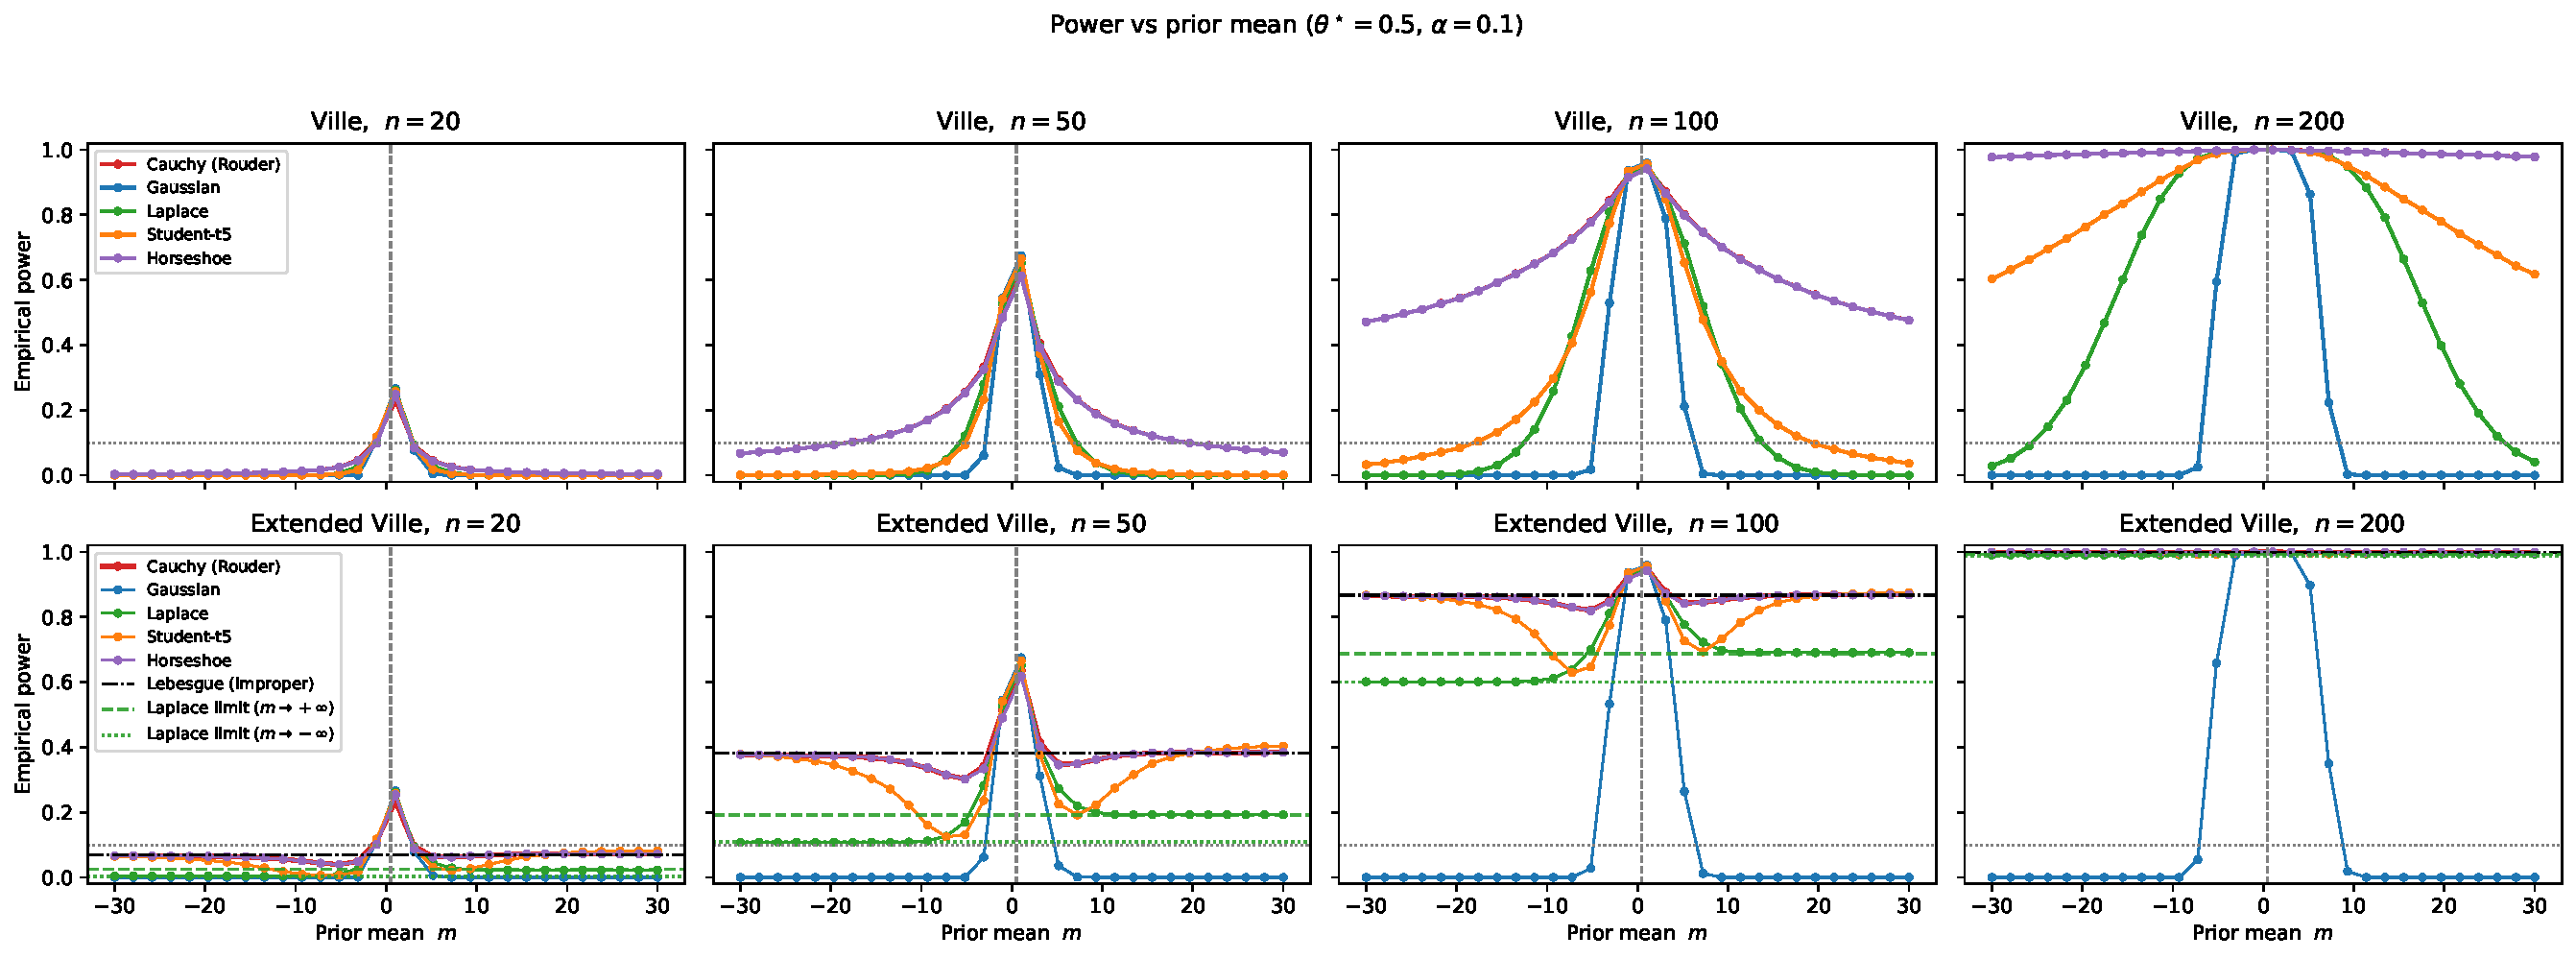
\includegraphics[width=1\linewidth, height=0.4\linewidth]{images/power_vs_m_priors_v5.pdf}
    \caption{Empirical power of the Ville (top row) and extended-Ville
    (bottom row) tests of \(H_0:\theta^\star=0\) under four proper
    priors of unit scale and varying location \(m\), at
    \(\theta^\star=0.5\) and \(\alpha=0.1\), for sample sizes
    \(n\in\{5,20,50,100,200\}\). Each panel uses
    \(B=10{,}000\) data replicates and \(B_{\mathrm{cal}}=100{,}000\)
    calibration replicates. The dashed vertical line marks the
    well-specified location \(m=\theta^\star\); the dotted horizontal
    line marks the level \(\alpha\); the dash-dotted black line in
    the bottom row marks the noninformative Lebesgue extended-Ville
    baseline, which is independent of \(m\)
    by construction. The Cauchy curve (red) reproduces the Rouder--JZS Bayes
    factor.}
    \label{fig:power_vs_m_priors}
\end{figure}

\subsubsection{Running Setup}
We fix the data-generating effect \(\theta^\star=0.5\) and the
significance level \(\alpha=0.1\), and consider sample sizes
\(n\in\{20,50,100,200\}\). For each prior shape \(\pi\) of unit scale,
each location \(m\) on a grid
\(\mathcal M=\{-30,-7,\ldots,30\}\), and each pair \((n,m)\), we draw
\(B=10{,}000\) independent datasets
\(Y_{1:n}^{(b)}\stackrel{\mathrm{iid}}{\sim}\mathcal N(\theta^\star,1)\)
and report the empirical Ville and extended-Ville rejection rates
\begin{equation}\label{eq:exp-power}
   \widehat{\mathrm{pow}}_{n,\alpha}^{V}(m)
   = \frac{1}{B}\sum_{b=1}^{B}
     \mathbf 1\!\bigl\{P_{n,0}^{V,\Pi_m}(Y_{1:n}^{(b)})\leq\alpha\bigr\},
   \qquad
   \widehat{\mathrm{pow}}_{n,\alpha}^{eV}(m)
   = \frac{1}{B}\sum_{b=1}^{B}
     \mathbf 1\!\bigl\{P_{n,0}^{eV,\Pi_m}(Y_{1:n}^{(b)})\leq\alpha\bigr\}.
\end{equation}
We compare four proper priors: Cauchy (C), Gaussian (G), Laplace (LP),
Student-\(t_5\) (T5), and the horseshoe-type density
\(\pi_{\mathrm{HS}}(\theta)=(4\pi)^{-1}\log(1+4/\theta^2)\),
the renormalised Carvalho-Polson-Scott upper bound \cite{Carvalho2010}, which has the same Cauchy-rate polynomial tail
and soft logarithmic spike at zero as the exact horseshoe and is
computationally more tractable. The Gaussian is the canonical
exponential-square benchmark and falls outside
Assumption~\ref{ass:tails}; %the Laplace satisfies Assumption~\ref{ass:tails}
%with \(\kappa>0\), \(\beta=0\); 
and Student-\(t_5\) and the horseshoe
satisfy it with \(\kappa=0\), \(\beta=6\) and \(\beta=2\) respectively.
The improper Lebesgue prior of Section~\ref{ssec:Leb} is included as a
noninformative baseline in the extended-Ville panels; it does not appear
in the Ville panels, since the Ville construction requires a proper prior.

The marginal likelihoods \(M_n^{\Pi_m}\) and the
calibration functions \(g_{0}^{(m)}\) are unavailable in closed form for
the four proper priors and are computed numerically: \(M_n^{\Pi_m}(u_n)\)
by adaptive Gauss--Kronrod quadrature in \(\theta\) on a grid in
\(u_n\in(-\sqrt n,\sqrt n)\) followed by linear interpolation, and the
calibration \(g_{0}^{(m)}\) by Monte Carlo under \(\Prob_0\) with
\(B_{\mathrm{cal}}=100{,}000\) replicates. A single \(\Prob_0\)-sample
of pairs \((Y_1^{(j)},Y_2^{(j)})\) is reused across the entire
\((m,\pi)\) grid by re-evaluating
\(M_2^{\Pi_m}(Y_1^{(j)},Y_2^{(j)})\) at each grid point. The Lebesgue
baseline uses the closed forms of Theorems~\ref{thm:Mn-Leb}
and \ref{thm:gLeb} and incurs no Monte Carlo error in the calibration.


\subsubsection{Interpretation}\label{ssec:exp-interp}

Figure~\ref{fig:power_vs_m_priors} confirms the qualitative picture
predicted by Theorems~\ref{thm:CSVille-divergence} and \ref{thm:recovery}, and refines it across sample sizes. We observe the following.

\emph{Prior-data agreement.} For every prior and every \(n\), the power
curves attain their maximum at \(m=\theta^\star\), where the prior is
correctly centred. At this location the heavier-tailed priors (Cauchy, Student-$t_5$ and Horseshoe) deliver power comparable to the Gaussian and Laplace priors;
the gain over the non-informative Lebesgue baseline is substantial at
small \(n\) and progressively erodes as \(n\) grows, since the data become more informative.

The contrast between the top and bottom rows of Figure~\ref{fig:power_vs_m_priors} is the essential message: under the classical Ville construction every proper prior is fragile, while the
extended-Ville construction with polynomial-tail priors enjoys
informative power gains under prior-data agreement and graceful reversion to the scale-invariant \(t\)-test under arbitrary prior-data conflict.

% =====================================================================
% Proposition: order-dependence of the anytime-valid stopping time.
% Slot in immediately before the permutation experiment in the data
% application / discussion section.
% =====================================================================

\subsection{Order-dependence of the anytime-valid stopping time}
\label{sec:order-dependence}

The fixed-sample $t$-test rejects on the basis of $(\bar y_{N},s_{N})$, a function of the unordered sample, and is therefore permutation-invariant. By contrast, the anytime-valid stopping time
\[
   \tau_{\alpha}(y_{1},\ldots,y_{N}) \;:=\; \inf\bigl\{n\ge 2 : P_{n}(y_{1:n}) \le \alpha\bigr\} \;\in\; \{2,\ldots,N\}\cup\{\infty\}
\]
is adapted to the filtration $\mathcal{F}_{n}=\sigma(Y_{1},\ldots,Y_{n})$ rather than to the exchangeable $\sigma$-algebra $\sigma(\{Y_{1},\ldots,Y_{N}\})$, so $\tau_{\alpha}$ is genuinely a function of the recruitment order. The next proposition records what is and is not preserved under permutation.

\begin{proposition}[Order-dependence and joint validity]
\label{prop:order-dependence}
Let $Y_{1},\ldots,Y_{N}\stackrel{\mathrm{iid}}{\sim}\mathcal{N}(\mu,\sigma^{2})$, let $(P_{n})_{n\ge 2}$ be either the classical Ville $p$-process $P_{n}^{V}=\min(1/M_{n}^{\Pi},1)$ for a proper prior $\Pi$ or an extended-Ville $p$-process $P_{n}^{eV}=g_{\Pi}(M_{n}^{\Pi})$ for a (possibly improper) prior $\Pi$, and let $\tau_{\alpha}$ be the associated stopping time.
\begin{enumerate}
\item[(i)] For every deterministic enrolment order $\sigma\in\mathcal{S}_{N}$,
   \[
      \Prob_{H_{0}}\bigl(\tau_{\alpha}(Y_{\sigma(1)},\ldots,Y_{\sigma(N)})<\infty\bigr)\;\le\;\alpha.
   \]
\item[(ii)] For a fixed realisation $(y_{1},\ldots,y_{N})$ the map $\sigma\mapsto\tau_{\alpha}(y_{\sigma(1)},\ldots,y_{\sigma(N)})$ is in general non-constant; in particular $\tau_{\alpha}$ is not measurable with respect to the unordered observation $\{y_{1},\ldots,y_{N}\}$, which is a complete sufficient statistic for $(\mu,\sigma^{2})$.
\item[(iii)] If $\sigma\sim\mathrm{Unif}(\mathcal{S}_{N})$ is drawn independently of the data, then
   \[
      \Prob_{H_{0},\sigma}\bigl(\tau_{\alpha}(Y_{\sigma(1)},\ldots,Y_{\sigma(N)})<\infty\bigr)\;\le\;\alpha,
   \]
   so the procedure remains anytime-valid under the joint randomisation.
\end{enumerate}
\end{proposition}

\begin{proof}
\begin{itemize}
\item[(i)] This is Ville's inequality applied to $(M_{n}^{\Pi})$ on the filtration $\mathcal{F}_{n}^{\sigma}=\sigma(Y_{\sigma(1)},\ldots,Y_{\sigma(n)})$, which is a non-negative supermartingale under $H_{0}$ for each fixed $\sigma$ (proper $\Pi$); the extended-Ville case is the analogous statement for the calibrated $p$-process \citep{wang2025extended}. 

\item[(ii)] This is immediate as $u_{n}=\sum_{i\le n}y_{i}/\sqrt{\sum_{i\le n}y_{i}^{2}}$ depends on which indices are included up to step $n$, hence on the order. 

\item[(iii)] This follows from (i) by Fubini, since
\[
   \Prob_{H_{0},\sigma}\bigl(\tau_{\alpha}<\infty\bigr) \;=\; \mathbb{E}_{\sigma}\bigl[\Prob_{H_{0}}(\tau_{\alpha}<\infty\mid\sigma)\bigr]\;\le\;\alpha.
\]
\end{itemize}
\end{proof}

The procedure is therefore valid under each fixed order, what varies across orders is the operational quantity $\tau_{\alpha}$ - the sample size at which we actually stop. For an exchangeable sample no single ordering is privileged, so we report a single dataset's anytime-valid performance via the permutation distribution of $\tau_{\alpha}$,
\begin{equation}\label{eq:perm-cdf}
   \widehat{F}_{\tau_{\alpha}}(t) \;=\; \frac{1}{B}\sum_{b=1}^{B}\mathbf{1}\bigl\{\tau_{\alpha}\bigl(y_{\sigma_{b}(1)},\ldots,y_{\sigma_{b}(N)}\bigr)\le t\bigr\}, \quad \sigma_{1},\ldots,\sigma_{B}\stackrel{\mathrm{iid}}{\sim}\mathrm{Unif}(\mathcal{S}_{N}).
\end{equation}

Two features of $\widehat{F}_{\tau_{\alpha}}$ are noteworthy.

\paragraph{Null calibration.} Under $H_{0}$, Proposition~\ref{prop:order-dependence}(iii) gives $\mathbb{E}\bigl[\widehat{F}_{\tau_{\alpha}}(N)\bigr]\le\alpha$, so the fraction of permutations rejecting by the full horizon is bounded by~$\alpha$ up to Monte-Carlo error of order $\sqrt{\alpha(1-\alpha)/B}$. This is a finite-sample diagnostic that the implementation is correctly calibrated.

\paragraph{Matched-pair efficiency comparison.} Comparing two procedures (e.g.\ classical Ville and extended Ville) on the same permutation $\sigma_{b}$ yields the matched-pair difference $\tau_{\alpha}^{V}(\sigma_{b})-\tau_{\alpha}^{eV}(\sigma_{b})$, which is non-negative whenever both stop and removes the dataset-level variation contributing to the marginal distributions. A sign test on the matched differences supplies a calibrated test of $H_{0}^{*}\colon\mathbb{E}[\tau_{\alpha}^{V}-\tau_{\alpha}^{eV}]=0$ against $H_{1}^{*}\colon\tau_{\alpha}^{eV}<\tau_{\alpha}^{V}$ stochastically.

% We use $\widehat{F}_{\tau_{\alpha}}$ and the matched-pair gain throughout Section~\ref{sec:neurovault} to summarise the operational behaviour of the anytime-valid $t$-test on the Bo et al.~\cite{bo2024systems} sample.

\subsection{Real-data application: Bo et al.\ emotion-regulation contrast}
\label{sec:neurovault}
We illustrate the procedure on a publicly available neuroimaging dataset from
the systems-identification study of \cite{bo2024systems}, accessed via the
NeuroVault repository \citep{gorgolewski2015neurovault} as collection
\textsc{16266}.\footnote{\url{https://neurovault.org/collections/16266/}} The
study examines the brain bases of cognitive emotion regulation; the
contrast of interest is the per-subject \emph{reappraisal-versus-look}
activation map, available as a separate three-dimensional NIfTI volume for
each participant. We treat each volume as the realisation of a per-subject
summary statistic, and apply the anytime-valid procedures to the resulting
sequence under recruitment order.

\paragraph{Data acquisition.}
We download the $N = 176$ subject-level contrast volumes from collection \textsc{16266} via the NeuroVault REST API. Each volume $\mathbf{V}_i$, $i = 1,\ldots,N$, is stored on a common MNI grid of dimensions
$79 \times 95 \times 79$ at $2 \times 2 \times 2 \mathrm{mm}^3$ resolution, with voxel intensities representing the test statistic of the contrast at that voxel in subject $i$. The values are unitless and span a range of
approximately $[-10, 40]$ across voxels and subjects.

\paragraph{ROI mask.}
A region-of-interest (ROI) mask $\mathcal{R}$ is required to reduce each volume to a scalar summary. In principle one would use a hypothesis-driven ROI in the prefrontal regions implicated in reappraisal \citep{buhle2014cognitive}; for the purposes of demonstrating the anytime-valid
machinery on real data, however, the precise choice of ROI is secondary, and we adopt a whole-brain mask defined as the set of non-zero voxels of the first subject's volume, resampled to each subject's grid via nearest-
neighbour interpolation when grids differ. The mask contains approximately
$3 \times 10^5$ voxels.

\paragraph{Per-subject summary.}
For each subject $i$, we summarise the volume $\mathbf{V}_i$ within the
mask $\mathcal{R}$ by its sample mean,
\begin{equation}
\label{eq:y_obs_def}
  Y_i \;:=\; \frac{1}{|\mathcal{R}|}\sum_{v \in \mathcal{R}} V_i(v),
  \qquad i = 1, \ldots, N,
\end{equation}
where $V_i(v)$ denotes the value of $\mathbf{V}_i$ at voxel $v$. Non-finite
voxels (arising from masking outside the imaged volume) are excluded from
the sum and the denominator adjusted accordingly. The resulting sequence
$Y_{1:N} = (Y_1, \ldots, Y_N) \in \mathbb{R}^N$ is the input to the
anytime-valid procedures.

\paragraph{Modelling assumption.}
We model $Y_i \stackrel{\mathrm{iid}}{\sim} \mathcal{N}(\mu, \sigma^2)$
with both $\mu$ and $\sigma^2$ unknown, and test the standardised
hypothesis
\[
  H_0:\; \theta^\star = \mu/\sigma = 0
  \quad\text{versus}\quad
  H_1:\; \theta^\star \neq 0.
\]
The iid Gaussian assumption is standard at the group level in neuroimaging
\cite{penny2012comparing}; the scale-invariant standardisation $\theta^\star =
\mu/\sigma$ is what the procedures the proposed test, by construction. With the observed sample we compute the sample mean $\overline{Y}_N$, sample standard deviation $S_N$, and the sample Sharpe ratio $\widehat\theta_N = \overline{Y}_N / S_N$; on this dataset $\widehat\theta_N \approx 1.69$, indicating substantial evidence against $H_0$ at the full sample size.

\paragraph{Recruitment order and sequential analysis.}
The NeuroVault collection does not preserve the temporal order in which subjects were recruited; we treat the order in which the volumes appear in the collection as a stand-in for recruitment order. This is the order in which the anytime-valid p-process $(P_n)_{n \geq 2}$ is updated. The substantive interpretation is then,  if the experimenters had applied an anytime-valid procedure during data collection and stopped at the first $n$ for which $P_n \leq \alpha$, what would the operating characteristics have been? We quantify this question by computing the running anytime-valid p-value under several priors and comparing the first-rejection time of the classical Ville and the extended Ville constructions. 

\subsubsection{Results: first-rejection times}
\label{sec:neurovault-results}

We apply the anytime-valid procedures of
Sections~\ref{sec:closedform}--\ref{sec:bdd-influence} to the preprocessed sequence $Y_{1:N}$ at level $\alpha = 0.05$, under five proper priors of unit scale (Cauchy, Gaussian, Laplace, Student-$t_5$,
horseshoe) and the improper Lebesgue prior. To probe robustness under prior-data conflict, each proper prior is shifted to four locations
$m \in \{0, 3, 10, 30\}$, ranging from approximately well-specified
($m = 0$, close to the sample mean of $Y_{1:N}$) to strongly conflicting
($m = 30$, far in the right tail of the observed values). For every
$(\text{prior}, m)$ combination we compute both the classical Ville
$p$-process $P_n^{V} = \min(1/M_n^{\Pi}, 1)$ and the extended-Ville
$p$-process $P_n^{eV} = g^{\Pi}(M_n^{\Pi})$, where $g^{\Pi}$ is calibrated
under $H_0$ at $n = 2$ via Monte Carlo with $B_{\mathrm{cal}} = 10^5$
replicates. The first-rejection time under each construction is then
\[
  \tau^{\bullet}(\Pi, m)
  \;:=\;
  \inf \bigl\{ n \in \{2, \ldots, N\} :\, P_n^{\bullet} \leq \alpha \bigr\},
  \qquad \bullet \in \{V, eV\},
\]
with $\tau^{\bullet}(\Pi, m) = \infty$ if no crossing occurs within $N$ subjects.


\begin{figure}
    \centering
    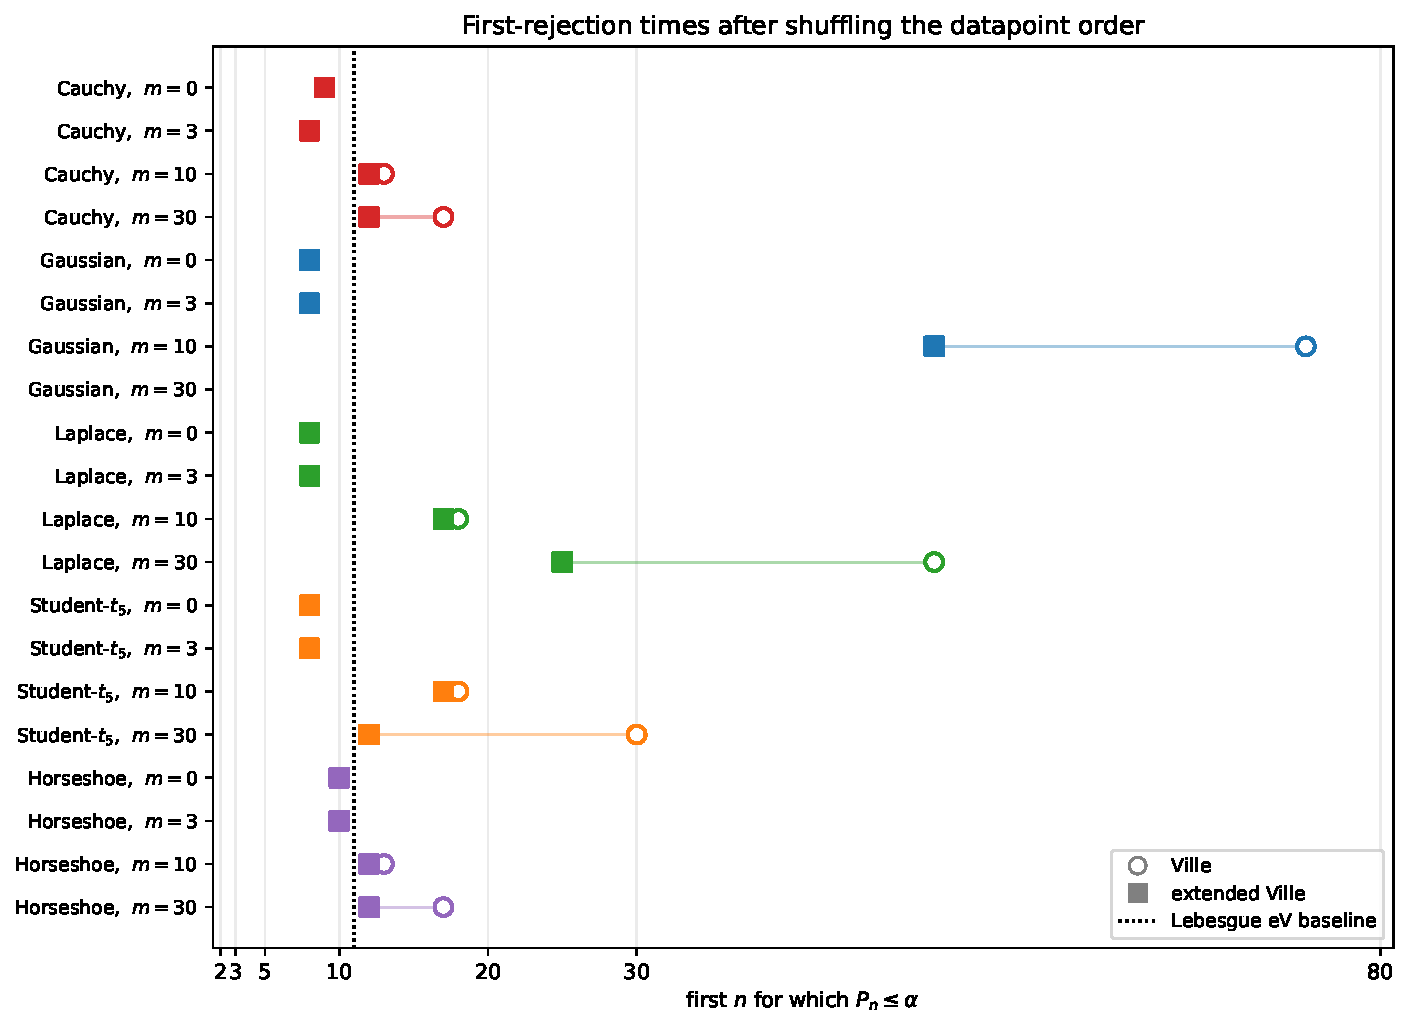
\includegraphics[width=\linewidth]{images/neurovault_first_rejection_shuffled.pdf}
    \caption{First $n$ for which the p-process crosses the threshold $\alpha = 0.05$}
    \label{fig:neurovault-first-rejection}
\end{figure}

Figure~\ref{fig:neurovault-first-rejection} displays
$(\tau^{V}, \tau^{eV})$ for each of the $5 \times 4 = 20$
$(\text{prior}, m)$ combinations. Filled squares give the extended-Ville first-rejection time; open circles give the classical Ville first-rejection time; thin connector segments join the two when both procedures reject within $N$ subjects. The dotted vertical line marks the Lebesgue extended-Ville baseline $\tau^{eV}(\Pi_{\mathrm{Leb}}) = 2$, which is the non-informative anytime-valid $t$-test of \cite{Lai1976} calibrated under the extended Ville inequality of \cite{wang2025extended}.

\paragraph{Classical Ville under conflict.}
The classical Ville first-rejection times $\tau^{V}(\Pi, m)$ deteriorate visibly at $m = 30$ for the polynomial-tail priors (the
horseshoe and Cauchy first reject at $n = 17$ and $n = 12$ respectively, against $\tau^{eV} = 2$ for both) and for the Laplace prior at $m = 30$ ($\tau^{V} \approx 30$). For the Gaussian prior at $m=30$, the classical Ville doesn't cross the threshold. This is the empirical manifestation of Theorem~\ref{thm:CSVille-divergence}: under prior-data conflict, the Ville construction is fragile, and informative priors do not save it. The corresponding extended-Ville procedures, by contrast, are robust to the same conflict, illustrating the central operational consequence of the extended Ville inequality in this setting.


\section{Conclusion}

This report developed the anytime-valid $t$-test with informative priors in the
unknown-variance setting. On the scale-invariant filtration we obtained closed
forms for the mixture statistic under the Lebesgue prior, recovering the
scale-invariant $t$-statistic, and under the one-sided exponential tilt in terms
of the parabolic cylinder function $D_{-n}$, and we identified the directional
limits of the symmetric Laplace mixture with these tilts.

The main result is a trichotomy governed by the prior's tail relative to the
Gaussian envelope $e^{-n\theta^2/2}$. Polynomial-tail priors give the
bounded-influence property, i.e. under the extended-Ville calibration the procedure reverts to the non-informative benchmark as prior-data conflict grows, whereas the classical Ville confidence sequence is fragile for every proper prior. Exponential-tail priors such as Laplace sit on the borderline, converging to a non-trivial limit that keeps a directional signal rather than reverting. For sub-Gaussian priors our
simulations indicate that the procedure fails to reject regardless of the data. We
aim to develop the theory for the sub-Gaussian regime, which would complete the trichotomy. We also found that the known-variance Hausdorff data-conflict limit has no analogue here, since $u_n$ is bounded and $\theta^\star$ is a ratio rather than a location.

The informative procedures used here rely on Monte Carlo calibration, so sharper or closed-form calibration would be useful; this is also
the main practical drawback of the method, since the calibration must be
recomputed whenever the prior or its location changes, and the per-evaluation cost of the mixture statistic by quadrature is non-trivial at large $n$ and near the data-conflict boundary $|u_n| \to \sqrt{n}$, where the integrand becomes sharply peaked. Scenarios with sequential monitoring under genuine prior information arise in
many real-life settings, and demonstrating the method on such datasets through concrete experiments is a natural next step.

\bibliography{bayesanytimettest}
\bibliographystyle{alpha}



\appendix
\section*{Appendix}
\section{Closed-form expression for the scale-invariant likelihood ratio}\label{app:a}
In this section, for the sake of completeness, we provide the detailed calculation behind equation~\eqref{eq:hthetadef}. The result is taken from \cite{Wang2025}, which expresses the scale-invariant likelihood ratio $L_n$ in closed form. Throughout, fix $y_{1:n}=(y_1,\dots,y_n)\in\mathbb{R}^n$ and set
\[
  T \;:=\; \sum_{i=1}^{n}y_i,
  \qquad
  S \;:=\; \sum_{i=1}^{n}y_i^{2},
  \qquad
  u_n \;:=\; u_n(y_{1:n}) \;=\; \frac{T}{\sqrt{S}}.
\]
We work on the event $\{S>0\}$, which has $P_{\theta,\sigma}$-probability
one for every $(\theta,\sigma)$ and every $n\geq 1$.

\begin{proposition}
\label{prop:scale-invariant}
Let $f_{n,\theta,\sigma}$ denote the joint density of
$Y_{1:n}\stackrel{\mathrm{iid}}{\sim}\mathcal{N}(\theta\sigma,\sigma^{2})$.
Then for every $\theta\in\mathbb{R}$,
\begin{equation}
\label{eq:integratedlik}
\int_{0}^{\infty} f_{n,\theta,\sigma}(y_{1:n})\,\sigma^{-1}\,\diff\sigma
\;=\;
\frac{\Gamma(n/2)}{2\,\pi^{n/2}\,S^{\,n/2}}\,
e^{-n\theta^{2}/2}\, A_n(\theta u_n).
\end{equation}
Consequently, with $h_{\theta,n}(y_{1:n}):=e^{-n\theta^{2}/2}A_n(\theta u_n)$, $L_n(y_{1:n};\theta_0,\theta) = \frac{h_{\theta,n}(y_{1:n})}{h_{\theta_0,n}(y_{1:n})}$, 
where $L_n(y_{1:n};\theta_0,\theta)$ and $A_n(z)$ are as defined in equations~\eqref{eq:hthetadef} and ~\eqref{eq:Andef} respectively.

\end{proposition}

\begin{proof}
By independence,
\[
f_{n,\theta,\sigma}(y_{1:n})
= (2\pi\sigma^{2})^{-n/2}\exp\!\left(
   -\frac{1}{2\sigma^{2}}\sum_{i=1}^{n}(y_i-\theta\sigma)^{2}\right).
\]
Expanding the quadratic,
\[
\sum_{i=1}^{n}(y_i-\theta\sigma)^{2}
= S - 2\theta\sigma T + n\theta^{2}\sigma^{2},
\]
so that
\[
f_{n,\theta,\sigma}(y_{1:n})
= (2\pi)^{-n/2}\,\sigma^{-n}\,
  e^{-n\theta^{2}/2}\,
  \exp\!\left(-\frac{S}{2\sigma^{2}} + \frac{\theta T}{\sigma}\right).
\]
The factor $e^{-n\theta^{2}/2}$ has been pulled outside because it does not depend on $\sigma$. Multiplying this by $\sigma^{-1}$ and integrating,
\begin{equation}
\label{eq:Ipre}
\int_{0}^{\infty}\! f_{n,\theta,\sigma}(y_{1:n})\sigma^{-1}\diff\sigma
= (2\pi)^{-n/2}\,e^{-n\theta^{2}/2}\,
\int_{0}^{\infty}\!\sigma^{-n-1}
   \exp\!\left(-\frac{S}{2\sigma^{2}}+\frac{\theta T}{\sigma}\right)\diff\sigma.
\end{equation}
Suppose we call the integral part $J_n(\theta)$. For $\sigma>0$, introduce the change of variables
\[
v \;=\; \frac{S}{2\sigma^{2}},
\qquad\text{equivalently}\qquad
\sigma \;=\; \sqrt{\frac{S}{2v}},
\]
which is a $C^{1}$-diffeomorphism from $(0,\infty)$ onto $(0,\infty)$ (sending
$\sigma\to 0^{+}$ to $v\to\infty$ and vice versa). The Jacobian and basic
identities are
\[
\frac{\diff\sigma}{\diff v}
= -\tfrac{1}{4}\sqrt{2S}\,v^{-3/2},
\qquad
\frac{1}{\sigma}=\sqrt{\frac{2v}{S}},
\qquad
\sigma^{-n-1}=\left(\frac{2v}{S}\right)^{(n+1)/2}.
\]
A key observation is
\[
\frac{\theta T}{\sigma}
\;=\;\theta T\sqrt{\frac{2v}{S}}
\;=\;\theta \cdot \frac{T}{\sqrt{S}}\cdot \sqrt{2v}
\;=\;\theta\, u_n \sqrt{2v},
\]
so the exponent becomes a function of $u_n$ rather than of $T$ and $S$
separately. Reversing the integration limits and absorbing the resulting
sign,
\begin{align*}
J_n(\theta)
& = \frac{\sqrt{2S}}{4}
\int_{0}^{\infty}\!\left(\frac{2v}{S}\right)^{\!(n+1)/2}\! v^{-3/2}\,
e^{-v + \theta u_n\sqrt{2v}}\,\diff v\\
& = \frac{2^{(n+2)/2}}{4}\, S^{-n/2}\,
   \int_{0}^{\infty}\! v^{n/2-1}\,
   e^{-v + \theta u_n\sqrt{2v}}\,\diff v\\
& = 2^{\,n/2-1}\, S^{-n/2}\, \Gamma(n/2)\, A_n(\theta u_n)
\end{align*}
where the last equality is the definition~\eqref{eq:Andef} of $A_n$. Thus,
\begin{align*}
\int_{0}^{\infty} f_{n,\theta,\sigma}(y_{1:n})\sigma^{-1}\diff\sigma
&= (2\pi)^{-n/2}\,2^{\,n/2-1}\,\Gamma(n/2)\,S^{-n/2}\,
   e^{-n\theta^{2}/2}\,A_n(\theta u_n)\\
&= \frac{2^{\,n/2-1}}{2^{\,n/2}\,\pi^{n/2}}\,\Gamma(n/2)\,S^{-n/2}\,
   e^{-n\theta^{2}/2}\,A_n(\theta u_n)\\
&= \frac{\Gamma(n/2)}{2\,\pi^{n/2}}\,S^{-n/2}\,
   e^{-n\theta^{2}/2}\,A_n(\theta u_n),
\end{align*}
which is exactly~\eqref{eq:integratedlik}. The prefactor $\Gamma(n/2)/(2\pi^{n/2})\cdot S^{-n/2}$
in~\eqref{eq:integratedlik} depends on $y_{1:n}$ only through $S$ and is independent of $\theta$. It therefore cancels in the ratio:
\[
L_n(y_{1:n};\theta_0,\theta)
=\frac{\int_{0}^{\infty}\! f_{n,\theta,\sigma}\,\sigma^{-1}\diff\sigma}
      {\int_{0}^{\infty}\! f_{n,\theta_0,\sigma}\,\sigma^{-1}\diff\sigma}
=\frac{e^{-n\theta^{2}/2}\,A_n(\theta u_n)}
      {e^{-n\theta_0^{2}/2}\,A_n(\theta_0 u_n)}
=\frac{h_{\theta,n}(y_{1:n})}{h_{\theta_0,n}(y_{1:n})},
\]
proving~\eqref{eq:hthetadef}. 
\end{proof}

\paragraph{$A_n$ as the chi MGF.} Let $R_n$ be a random variable which follows the $\chi_n$ distribution. Then it has density
\[
p_{R_n}(r)
=\frac{1}{2^{\,n/2-1}\,\Gamma(n/2)}\,
  r^{\,n-1}\,e^{-r^{2}/2}\,\1_{\{r\geq 0\}},
\]
which can be derived from the fact that $R_n^{2}\sim\chi^{2}_n$ has the $\mathrm{Gamma}(n/2,1/2)$ density. Substituting
$y=r^{2}/2$ (so $r=\sqrt{2y}$ and $\diff r=\diff y/\sqrt{2y}$),
\allowdisplaybreaks
\begin{align*}
\E\!\left[e^{zR_n}\right]
&=\frac{1}{2^{\,n/2-1}\Gamma(n/2)}
  \int_{0}^{\infty}\! r^{\,n-1}\,e^{-r^{2}/2 + zr}\,\diff r\\
&=\frac{1}{2^{\,n/2-1}\Gamma(n/2)}
  \int_{0}^{\infty}\! (2y)^{(n-1)/2}\,e^{-y+z\sqrt{2y}}\,\frac{\diff y}{\sqrt{2y}}\\
&=\frac{1}{2^{\,n/2-1}\Gamma(n/2)}\cdot 2^{\,n/2-1}
  \int_{0}^{\infty}\! y^{\,n/2-1}\,e^{-y+z\sqrt{2y}}\,\diff y\\
&=\frac{1}{\Gamma(n/2)}
  \int_{0}^{\infty}\! y^{\,n/2-1}\,e^{-y+z\sqrt{2y}}\,\diff y
  \;=\; A_n(z),
\end{align*}
Finiteness for all $z\in\mathbb{R}$ follows from $-r^{2}/2+zr\leq -r^{2}/4+z^{2}$.

\paragraph{Sharpe-ratio form of $u_n$ and boundedness.} With $\overline{Y}_n=T/n$ and
$S_n^{2}=(n-1)^{-1}\sum_{i=1}^{n}(y_i-\overline{Y}_n)^{2}$, the standard
identity $\sum(y_i-\overline{Y}_n)^{2}=S-n\overline{Y}_n^{2}=S-T^{2}/n$
gives
\[
S \;=\; (n-1)\,S_n^{2} \;+\; \frac{T^{2}}{n}.
\]
The sample Sharpe ratio is
$\widehat{\theta}_n=\overline{Y}_n/S_n=T/(nS_n)$, hence
$T=nS_n\widehat{\theta}_n$ and $T^{2}=n^{2}S_n^{2}\widehat{\theta}_n^{2}$, so
\[
S \;=\; S_n^{2}\!\left((n-1)+n\widehat{\theta}_n^{2}\right),
\qquad
u_n \;=\; \frac{T}{\sqrt{S}}
\;=\; \frac{n\,\widehat{\theta}_n}{\sqrt{(n-1)+n\widehat{\theta}_n^{2}}},
\]


\section{Extended martingale property of the one-sided exponential tilt}
\label{app:extended-mg}
This appendix supplies the proof of the claim made that the process \((M_n^{(\kappa)}(Y_{1:n}))_{n\geq 2}\) defined in~\eqref{eq:Mkappa-def} is a non-negative extended martingale under \(H_0:\theta^\star=0\). The
argument is the t-test specialisation of the disintegration construction of Lemma $5.4$ of \cite{Wang2025}; we reproduce it in our notation for completeness.

\subsection{Extended martingales}

We first recall the relevant definition. A process \((X_n)_{n\geq n_0}\)
adapted to a filtration \((\mathcal{F}_n)_{n\geq n_0}\) and taking values
in \([0,\infty]\) is an extended non-negative martingale under
\(\mathbb{P}_0\) if,
\begin{enumerate}
\item[(i)] \(X_n<\infty\) \(\mathbb{P}_0\)-a.s. for every \(n\geq n_0\)
\item[(ii)] for every \(n\geq n_0\),
\(\E_0[X_{n+1}\mid \mathcal{F}_n]=X_n\) \(\mathbb{P}_0\)-a.s.
\item[(iii)] \(\E_0[X_{n_0}]\) may be infinite.
\end{enumerate}
The only difference from an ordinary non-negative martingale is the
relaxation of the integrability requirement (iii). The extended Ville
inequality (Proposition~\ref{prop:eville}) still applies, with the conclusion \(\mathbb{P}_0(\sup_n X_n\geq c)\leq \E_0[\min(X_{n_0}/c,1)]\) replacing the classical bound \(1/c\); the latter follows from \(\E_0[X_{n_0}]\leq 1\) and is unavailable when \(\E_0[X_{n_0}]=\infty\).

\subsection{Setting and statement}

Recall the setup of Section~\ref{sec:exptilt}. We work under \(H_0:\theta^\star=0\),
equivalently \(Y_1,Y_2,\ldots\stackrel{\mathrm{iid}}{\sim}\mathcal{N}(0,\sigma^2)\)
for some unknown \(\sigma>0\). The scale-invariant filtration is
\(\mathcal{F}_n=\sigma(Z_1,\ldots,Z_n)\) with \(Z_i=Y_i/|Y_1|\), the
scale-invariant likelihood ratio \(L_n(y_{1:n};0,\theta)\) is given by
\eqref{eq:hthetadef}, and the joint \(\sigma\)-finite exponential-tilt prior on \((\theta,\sigma)\) is
\[
\pi_\kappa(\theta,\sigma)\,\dd\theta\,\dd\sigma
\;=\;\frac{\exp(-\kappa(\theta-m))}{\sqrt{2\pi}\,\sigma}\,
\dd\theta\,\dd\sigma,
\qquad \kappa\in\mathbb{R},\ m\in\mathbb{R}.
\]
The marginal likelihood \eqref{eq:Mkappa-def} can be rewritten in terms of the scale-invariant likelihood ratio as follows. Disintegrating the joint prior into its \(\theta\)-marginal (an improper density on \(\mathbb{R}\)) and the right-Haar measure on \(\sigma\), and using the identity \eqref{eq:scale-inv-LR}. 

\begin{equation}\label{eq:Mkappa-as-mixture}
M_n^{(\kappa)}(y_{1:n})
\;=\;\int_\mathbb{R} L_n(y_{1:n};0,\theta)\,\nu_\kappa(\dd\theta)
\;\times\; \int_0^\infty f_{n,0,\sigma}(y_{1:n})\,\sigma^{-1}\,\dd\sigma,
\end{equation}
where \(\nu_\kappa(\dd\theta) := \exp(-\kappa(\theta-m))\,\dd\theta\) is
the \(\sigma\)-finite \(\theta\)-marginal of the joint prior. The
second factor in \eqref{eq:Mkappa-as-mixture} is the null marginal
density of \(Y_{1:n}\) integrated against the right-Haar prior, which is
positive and finite \(\mathbb{P}_0\)-a.s. by the calculation in Appendix~\ref{app:a}. The whole \(\mathbb{P}_0\)-a.s.-finiteness of \(M_n^{(\kappa)}\) was established in Section~\ref{sec:exptilt} by the Gaussian-envelope argument.

\begin{proposition}\label{prop:extended-mg}
Under \(H_0:\theta^\star=0\), the process
\((M_n^{(\kappa)}(Y_{1:n}))_{n\geq 2}\) is an extended non-negative
martingale with respect to the scale-invariant filtration
\((\mathcal{F}_n)_{n\geq 2}\).
\end{proposition}


\begin{proof}
The proof has three steps. We first show that, for every fixed $\theta$,
the scale-invariant likelihood ratio $L_n(\,\cdot\,;0,\theta)$ is itself a
non-negative martingale of mean one on the scale-invariant filtration. We then
integrate this pointwise martingale against the $\sigma$-finite measure
$\nu_\kappa$ to obtain the martingale property of $M_n^{(\kappa)}$, and finally
check that the unconditional first moment is infinite, which is what makes the process an extended martingale.

\paragraph{Step 1: $L_n$ is a non-negative martingale on $\mathcal{F}_n$.}
The filtration $\mathcal{F}_n = \sigma(Z_1,\dots,Z_n)$ with $Z_i = Y_i/|Y_1|$
is the smallest one that retains every scale-invariant function of the data
$Y_{1:n}$ and discards the rest. The scale-invariant likelihood ratio
\eqref{eq:Ln-mg} depends on $Y_{1:n}$ only through $(Z_1,\dots,Z_n)$, by its
right-Haar representation; equivalently, it is the likelihood ratio between
the laws of $(Z_1,\dots,Z_n)$ under $\mathbb{P}_\theta$ and $\mathbb{P}_0$,
which are two genuine probability measures on the maximal invariant. As the
likelihood ratio between two probability measures with respect to a common
filtration, $(L_n(Y_{1:n};0,\theta))_{n\geq 1}$ is automatically a non-negative
martingale of mean one under the denominator measure $\mathbb{P}_0$
\citep[Cor.~4.6]{Wang2025}. That is, for every $n\geq 1$ and every
$\theta\in\mathbb{R}$,
\begin{equation}\label{eq:Ln-mg}
   \mathbb{E}_0\!\left[L_{n+1}(Y_{1:(n+1)};0,\theta)\,\big|\,\mathcal{F}_n\right]
   \;=\; L_n(Y_{1:n};0,\theta)
   \qquad\mathbb{P}_0\text{-a.s.,}
\end{equation}
and $\mathbb{E}_0[L_n(Y_{1:n};0,\theta)] = 1$ for every $n\geq 1$.

\paragraph{Step 2: martingale property of $M_n^{(\kappa)}$.}
By the right-Haar disintegration of Equation~\eqref{eq:Mkappa-as-mixture}, the marginal likelihood $M_n^{(\kappa)}$ can be written, on the maximal invariant,
as the $\nu_\kappa$-mixture of the scale-invariant likelihood ratios:
\begin{equation}\label{eq:M-as-mixture-Ln}
   M_n^{(\kappa)}(y_{1:n})
   \;=\; C_n(y_{1:n})\int_\mathbb{R} L_n(y_{1:n};0,\theta)\,\nu_\kappa(\dd\theta),
\end{equation}
where $C_n(y_{1:n}) = \int_0^\infty f_{n,0,\sigma}(y_{1:n})\,\sigma^{-1}\,\dd\sigma$
is the right-Haar null marginal and $\nu_\kappa(\dd\theta) = e^{-\kappa(\theta-m)}\,\dd\theta$
is the $\sigma$-finite $\theta$-marginal of the joint prior. Both factors on
the right-hand side are $\mathcal{F}_n$-measurable, $L_n$ by Step~1 and $C_n$ because it depends on $y_{1:n}$ only
through $\sum y_i^2$ via the formula
$C_n(y_{1:n}) = \Gamma(n/2)\,(2\pi^{n/2})^{-1}\,(\sum y_i^2)^{-n/2}$, which can be rewritten as
$|Y_1|^{-n}\,\Gamma(n/2)\,(2\pi^{n/2})^{-1}\,(\sum_{i=1}^n Z_i^2)^{-n/2}$. The term $|Y_1|^{-n}$ is not $\mathcal{F}_n$-measurable in isolation, but it is absorbed into the change of variables from $(Y_1,\dots,Y_n)$ to
$(Y_1; Z_2,\dots,Z_n)$ that defines the law of the maximal invariant, and
what remains \emph{is} a function of $(Z_1,\dots,Z_n)$ alone (see
\cite[proof of Cor.~4.6]{Wang2025}). We may therefore work directly with the
mixture process $\widetilde M_n := \int L_n(\cdot;0,\theta)\,\nu_\kappa(\dd\theta)$
on $\mathcal{F}_n$, and recover $M_n^{(\kappa)} = C_n\,\widetilde M_n$ at the
end.

\smallskip\noindent\emph{(i) Finiteness.}
By the Gaussian-envelope argument of Section~\ref{sec:exptilt},
$\widetilde M_n(y_{1:n})$ is finite for every $y_{1:n}$ with $\sum y_i^2 > 0$,
and hence $M_n^{(\kappa)}(Y_{1:n}) < \infty$ $\mathbb{P}_0$-a.s.

\smallskip\noindent\emph{(ii) Conditional expectation.}
The integrand $L_{n+1}(Y_{1:(n+1)};0,\theta)$ is non-negative and, for every
fixed $Y_{1:n}$, integrable against $\nu_\kappa$ by the same Gaussian-envelope
argument. Tonelli's theorem applies and lets us swap the conditional
expectation with the $\nu_\kappa$-integral. Using the pointwise martingale
property \eqref{eq:Ln-mg} pointwise in $\theta$,
\begin{align}
   \mathbb{E}_0\!\left[\widetilde M_{n+1}\,\big|\,\mathcal{F}_n\right]
   &= \mathbb{E}_0\!\left[\int_\mathbb{R} L_{n+1}(Y_{1:(n+1)};0,\theta)\,
       \nu_\kappa(\dd\theta)\,\Big|\,\mathcal{F}_n\right]\notag\\
   &= \int_\mathbb{R} \mathbb{E}_0\!\left[L_{n+1}(Y_{1:(n+1)};0,\theta)\,\big|\,
       \mathcal{F}_n\right]\,\nu_\kappa(\dd\theta)\notag\\
   &\overset{\eqref{eq:Ln-mg}}{=} \int_\mathbb{R} L_n(Y_{1:n};0,\theta)\,
       \nu_\kappa(\dd\theta)
   \;=\; \widetilde M_n.
   \label{eq:M-tilde-mg}
\end{align}
This is the martingale identity for $\widetilde M_n$ on
$(\mathcal{F}_n)_{n\geq 2}$. To pass it to $M_n^{(\kappa)} = C_n\widetilde M_n$,
note that the ratio $C_{n+1}/C_n$ is exactly the (scale-invariant) conditional
density of $Z_{n+1}$ given $\mathcal{F}_n$ under $\mathbb{P}_0$, by the same right-Haar computation fom which we get \eqref{eq:M-as-mixture-Ln}  \cite[Cor.~4.6]{Wang2025}. Therefore $C_n$ enters
\eqref{eq:M-tilde-mg} as a multiplicative $\mathcal{F}_n$-measurable factor
on both sides, and \eqref{eq:M-tilde-mg} is equivalent to
\begin{equation}\label{eq:Mkappa-mg}
   \mathbb{E}_0\!\left[M_{n+1}^{(\kappa)}(Y_{1:(n+1)})\,\big|\,\mathcal{F}_n\right]
   \;=\; M_n^{(\kappa)}(Y_{1:n})
   \qquad\mathbb{P}_0\text{-a.s.}
\end{equation}
This is property (ii) of the extended-martingale definition.

\paragraph{Step 3: failure of unconditional integrability.}
We finally verify property (iii), $\mathbb{E}_0[M_n^{(\kappa)}] = \infty$, which
is what makes the process an extended martingale. By Tonelli's theorem
( since the integrand is non-negative) and Step~1,
\[
   \mathbb{E}_0\!\left[\widetilde M_n\right]
   = \int_\mathbb{R} \mathbb{E}_0\!\left[L_n(Y_{1:n};0,\theta)\right]\,
       \nu_\kappa(\dd\theta)
   = \int_\mathbb{R} 1\,\nu_\kappa(\dd\theta)
   = \nu_\kappa(\mathbb{R}) = +\infty,
\]
since $\nu_\kappa$ has infinite total mass for every $\kappa\in\mathbb{R}$
($\nu_0$ is Lebesgue measure on $\mathbb{R}$; for $\kappa\neq 0$, one of the
two tails of $e^{-\kappa(\theta-m)}$ diverges). Because $C_n > 0$
$\mathbb{P}_0$-a.s., the same conclusion holds for $M_n^{(\kappa)}$:
$\mathbb{E}_0[M_n^{(\kappa)}] = +\infty$. Thus $(M_n^{(\kappa)})_{n\geq 2}$ is
genuinely extended and is not a classical martingale.

\smallskip\noindent Combining Steps~1--3, $(M_n^{(\kappa)}(Y_{1:n}))_{n\geq 2}$
is an extended non-negative martingale under $\mathbb{P}_0$ with respect to
$(\mathcal{F}_n)_{n\geq 2}$.
\end{proof}

\begin{remark}
    The disintegration in \eqref{eq:Mkappa-as-mixture} is essential. If one attempted to mix \(L_n\) directly against an improper joint prior on \((\theta,\sigma)\) without first reducing to the scale-invariant filtration, the resulting process would in general fail even the pointwise martingale property, because the likelihood ratio
\(f_{n,\theta,\sigma}/f_{n,0,\sigma}\) at fixed \(\sigma\) is not a
martingale on the original filtration \(\sigma(Y_1,\ldots,Y_n)\) under
\(\mathbb{P}_0\) (it depends on \(\sigma\), which is unknown). The
right-Haar measure \(\sigma^{-1}\dd\sigma\) is precisely the unique
(up to constant) measure that, when integrated out, produces the
likelihood ratio of the maximal invariant, which is a
martingale on the scale-invariant filtration. This is the
group-invariance content of \cite{PerezOrtiz2024}; the above result puts together this fact, the pointwise martingale property,
and Tonelli to obtain the mixture martingale property.
\end{remark}





\section{Asymptotics of \(A_n\) and \(h_{\theta,n}\)}
The behaviour of \(M_n^{\Pi_0}\) at the boundary \(|u_n|\to\sqrt n\) is
governed by the asymptotics of \(A_n\). Recall \(A_n(z)=\E[e^{zR_n}]\)
with \(R_n\sim\chi_n\).

\begin{lemma}\label{lem:An-asymp}
As \(z\to+\infty\),
\(A_n(z)\sim \frac{2^{1-n/2}\sqrt{2\pi}}{\Gamma(n/2)}\,z^{n-1}e^{z^2/2}\),
and as \(z\to-\infty\),
\(A_n(z)\sim \frac{2^{1-n/2}\Gamma(n)}{\Gamma(n/2)}|z|^{-n}\).
\end{lemma}

\begin{proof}
Substituting \(r=\sqrt{2y}\) yields
\(A_n(z) = \frac{2^{1-n/2}}{\Gamma(n/2)}\,e^{z^2/2}\int_0^\infty
r^{n-1}e^{-(r-z)^2/2}\dd r\). The integrand has a unique maximum at
\(r=z\) with quadratic envelope; Laplace's method gives the
\(z\to+\infty\) asymptotic. For \(z=-s\to-\infty\), substitute
\(u=sr\) and apply dominated convergence to the integral
\(\int_0^\infty u^{n-1}e^{-u-u^2/(2s^2)}\dd u\to\Gamma(n)\).
\end{proof}

A direct corollary describes the behaviour of \(h_{\theta,n}(u)\) on
the boundary \(u\to\sqrt n\). For \(\theta>0\),
\begin{equation}\label{eq:h-asymp}
  h_{\theta,n}(u)\;=\;e^{-n\theta^2/2}A_n(\theta u)
  \;\sim\;\frac{2^{1-n/2}\sqrt{2\pi}}{\Gamma(n/2)}
   (\theta u)^{n-1}e^{-\theta^2(n-u^2)/2}
   \quad (\theta\to+\infty).
\end{equation}
At \(u=\sqrt n\) the Gaussian envelope disappears and
\(h_{\theta,n}(\sqrt n)\sim \frac{2^{1-n/2}\sqrt{2\pi}}{\Gamma(n/2)}
(\theta\sqrt n)^{n-1}\), which is integrable in \(\theta\) only for
\(n=1\). This explains, heuristically, why proper priors fail at the
boundary.





\end{document} 